% 导入配置
% \documentclass[lang = cn, scheme = chinese, thmcnt = section]{elegantbook}
% elegantbook      设置elegantbook文档类
% lang = cn        设置中文环境
% scheme = chinese 设置标题为中文
% thmcnt = section 设置计数器


%% 1.封面设置

\title{Algebra Chapter 0 - Paolo Aluffi - NoteBook}                % 文档标题

\author{若水}               % 作者

\myemail{ethanmxzhou@163.com} % 邮箱

\homepage{helloethanzhou.github.io} % 主页

\date{\today}               % 日期

\extrainfo{上善若水任方圆}   % 箴言

\logo{PiCreatures_happy.pdf}        % 设置Logo

\cover{阿基米德螺旋曲线.pdf}          % 设置封面图片

% 修改标题页的色带
\definecolor{customcolor}{RGB}{135, 206, 250} 
% 定义一个名为customcolor的颜色,RGB颜色值为(135, 206, 250)

\colorlet{coverlinecolor}{customcolor}     % 将coverlinecolor颜色设置为customcolor颜色

%% 2.目录设置
\setcounter{tocdepth}{3}  % 目录深度为3

%% 3.引入宏包
\usepackage[all]{xy}
\usepackage{bbm, svg, graphicx, float, extpfeil, amsmath, amssymb, mathrsfs, mathalpha, boondox-cal, boondox-calo, hyperref, graphicx, romannum, chemarrow, booktabs, fontspec, ctex}

%% 4.定义命令
\newcommand{\N}{\mathbb{N}}            % 自然数集合
\newcommand{\R}{\mathbb{R}}            % 实数集合
\newcommand{\C}{\mathbb{C}}  		   % 复数集合
\newcommand{\Q}{\mathbb{Q}}            % 有理数集合
\newcommand{\Z}{\mathbb{Z}}            % 整数集合
\newcommand{\F}{\mathbb{F}}
\newcommand{\sub}{\subset}             % 包含
\newcommand{\im}{\text{im }}           % 像
\newcommand{\lang}{\langle}            % 左尖括号
\newcommand{\rang}{\rangle}            % 右尖括号
\newcommand{\dis}{\displaystyle}
\newcommand{\cont}{\text{cont}}
\newcommand{\cha}{\text{char}}
\newcommand{\function}[5]{
	\begin{align*}
		#1:\begin{aligned}[t]
			#2 &\longrightarrow #3\\
			#4 &\longmapsto #5
		\end{aligned}
	\end{align*}
}                                     % 函数

\newcommand{\lhdneq}{%
	\mathrel{\ooalign{$\lneq$\cr\raise.22ex\hbox{$\lhd$}\cr}}} % 真正规子群

\newcommand{\rhdneq}{%
	\mathrel{\ooalign{$\gneq$\cr\raise.22ex\hbox{$\rhd$}\cr}}} % 真正规子群

\newcommand{\upiff}{\mathrel{\rotatebox[origin=c]{90}{$\iff$}}} % 竖着的等价

\newcommand{\Rmnum}[1]{\uppercase\expandafter{\romannumeral #1}}  %定义命令输入大写罗马数字
\newcommand{\rmnum}[1]{\romannumeral #1}  %定义命令输入小写罗马数字



% \begin{document}

\chapter{群论$\rm\Rmnum{1}$}

\begin{figure}[H]
	\centering
	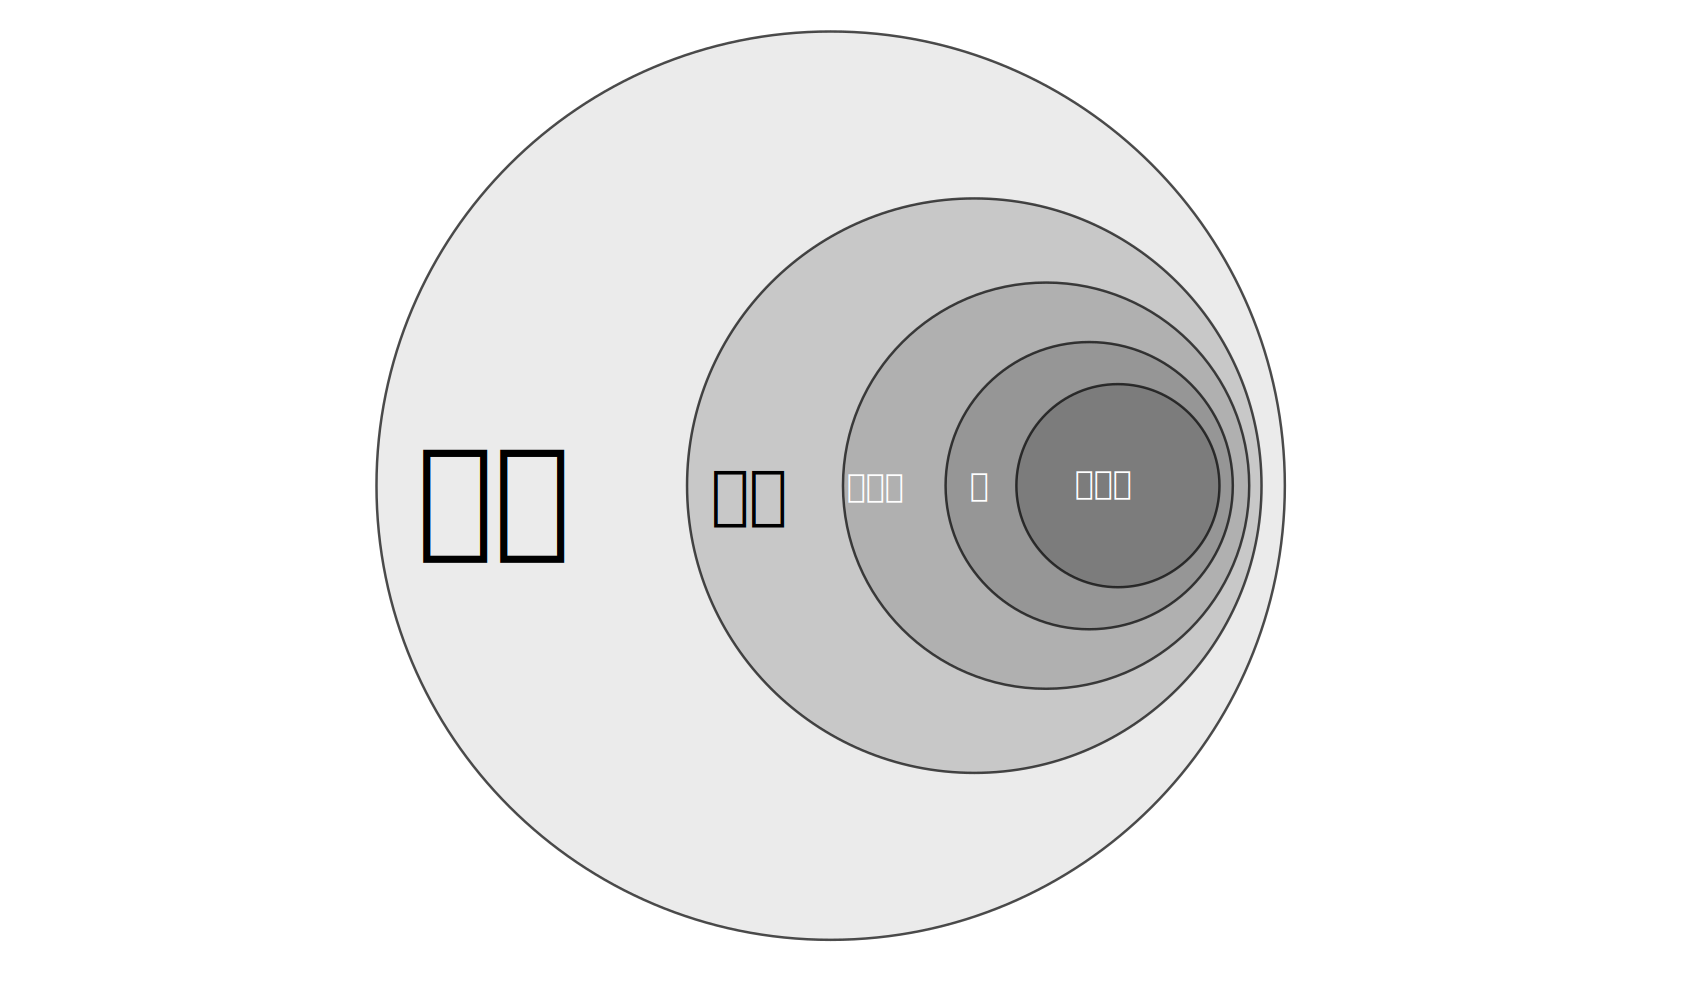
\includegraphics[scale = 0.4]{../figure/群}
	\caption{群的关系}
\end{figure}

\begin{table}[H]
	\centering
	\caption{群定义表}
	\begin{tabular}{|>{\centering\arraybackslash}m{1.5cm}|>{\centering\arraybackslash}m{1.5cm}|>{\centering\arraybackslash}m{1.5cm}|>{\centering\arraybackslash}m{1.5cm}|>{\centering\arraybackslash}m{1.5cm}|>{\centering\arraybackslash}m{1.5cm}|}
		\hline
		& \textbf{原群} & \textbf{半群} & \textbf{幺半群} & \textbf{群} & \textbf{交换群} \\
		\hline
		\textbf{封闭性} & $\checkmark$ & $\checkmark$ & $\checkmark$ & $\checkmark$ & $\checkmark$ \\
		\hline
		\textbf{结合律} & & $\checkmark$ & $\checkmark$ & $\checkmark$ & $\checkmark$ \\
		\hline
		\textbf{单位元} & & & $\checkmark$ & $\checkmark$ & $\checkmark$ \\
		\hline
		\textbf{逆元} & & & & $\checkmark$ & $\checkmark$ \\
		\hline
		\textbf{交换律} & & & & & $\checkmark$ \\
		\hline
	\end{tabular}
\end{table}

\section{群的定义}

\subsection{群和群胚}

\begin{definition}{群胚 groupoid}
	称范畴$\mathsf{C}$为群胚,如果其中任意态射均为同构态射。
\end{definition}

\begin{definition}{群 group}
	群是仅有一个对象的群胚。
\end{definition}

\subsection{定义}

\begin{definition}{原群 magma}
	称代数系统$(G,*)$为原群,如果$*$为二元运算$*:G\times G\to G$。
\end{definition}

\begin{definition}{半群 semigroup}
	称代数系统$(G,*)$为半群,如果二元运算$*:G\times G\to G$成立如下命题。
	\begin{enumerate}
		\item 结合律(associative):
		$$
		\forall g,h,k\in G,\quad (g*h)*k=g*(h*k)
		$$
	\end{enumerate}
\end{definition}

\begin{definition}{幺半群 monoid}
	称代数系统$(G,*)$为幺半群,如果二元运算$*:G\times G\to G$成立如下命题。
	\begin{enumerate}
		\item 单位元(identity element):
		$$
		\exists e\in G,\forall g\in G,\quad e*g=g*e=g
		$$
		\item 结合律(associative):
		$$
		\forall g,h,k\in G,\quad (g*h)*k=g*(h*k)
		$$
	\end{enumerate}
\end{definition}

\begin{definition}{群 group}
	称代数系统$(G,*)$为群,如果二元运算$*:G\times G\to G$成立如下命题。
	\begin{enumerate}
		\item 单位元(identity element):
		$$
		\exists e\in G,\forall g\in G,\quad e*g=g*e=g
		$$
		\item 逆元(inverse):$$
		\forall g\in G,\exists g^{-1},\quad g*g^{-1}=g^{-1}*g=e
		$$
		\item 结合律(associative):
		$$
		\forall g,h,k\in G,\quad (g*h)*k=g*(h*k)
		$$
	\end{enumerate}
\end{definition}

\begin{definition}{交换群 commutative group}
	称代数系统$(G,*)$为交换群,如果二元运算$*:G\times G\to G$成立如下命题。
	\begin{enumerate}
		\item 单位元(identity element):
		$$
		\exists e\in G,\forall g\in G,\quad e*g=g*e=g
		$$
		\item 逆元(inverse):$$
		\forall g\in G,\exists g^{-1},\quad g*g^{-1}=g^{-1}*g=e
		$$
		\item 结合律(associative):
		$$
		\forall g,h,k\in G,\quad (g*h)*k=g*(h*k)
		$$
		\item 交换律(commutative):
		$$
		\forall g,h\in G,\quad g*h=h*g
		$$
	\end{enumerate}
\end{definition}

\subsection{基本性质}

\begin{proposition}{单位元与逆元存在且存在唯一}
	\begin{enumerate}
		\item 单位元存在且存在唯一。
		\item 逆元存在且存在唯一。
	\end{enumerate}
\end{proposition}

\begin{proposition}{运算与逆元素按可换序}{2.1.3}
	对于群$(G,*)$,以及$g,h\in G$,成立$(g*h)^{-1}=h^{-1}*g^{-1}$。
\end{proposition}

\begin{proof}
	\begin{align*}
		&(g*h)*(h^{-1}*g^{-1})=g*(h*h^{-1})*g^{-1}=g*e*g^{-1}=e\\
		&(h^{-1}*g^{-1})*(g*h)=h*(g*g^{-1})*h^{-1}=h*e*h^{-1}=e
	\end{align*}
\end{proof}

\subsection{消去律}

\begin{theorem}{消去律 cancellation}{消去律}
	对于群$(G,*)$,以及任意$a,g,h\in G$,成立
	$$
	a*g=a*h\implies g=h\\
	g*a=h*a\implies g=h
	$$
\end{theorem}

\begin{proposition}
	对于群$(G,*)$,以及$g\in G$,成立$g*G=G$,其中
	$g*G=\{ g*h:h\in G \}$。
\end{proposition}

\begin{proof}
	首先,证明集合$g*G$中没有重复元素。任取$h_1,h_2\in G$,如果$g*h_1=g*h_2$,那么由消去律\ref{thm:消去律},$h_1=h_2$,于是集合$g*G$中没有重复元素。
	
	其次,任取$h\in G$,注意到
	$$
	h=e*h=(g*g^{-1})*h=g*(g^{-1}*h)\in g*G\implies G\sub g*G
	$$
	而显然$g*G\sub G$,因此$g*G=G$,命题得证!
\end{proof}

\subsection{交换群}

\begin{definition}{交换群 commutative group}
	称群$(G,*)$是可交换的,如果对于任意$g,h\in G$,成立$g*h=h*g$。
\end{definition}

\subsection{阶}

\begin{definition}{元素的阶 order}
	对于群$(G,*)$,定义元素$g\in G$的阶为
	$$
	|g|=\begin{cases}
		\min\{ n\in\N^*:g^n=e \},\qquad & \exists n\in\N^*, g^n=e\\
		\infty,\qquad & \forall n\in\N^*,g^n\ne e
	\end{cases}
	$$
\end{definition}

\begin{definition}{群的阶 order}
	定义有限群$(G,*)$的阶$|G|$为其元素的个数,无限群$(G,*)$的阶为$|G|=\infty$。
\end{definition}

\begin{proposition}
	如果群$(G,*)$对于任意$g\in G$,成立$g^2=e$,那么$G$为Abel群。
\end{proposition}

\begin{proof}
	由命题\ref{pro:2.1.3}
	$$
	g*h=g^{-1}*h^{-1}=(h*g)^{-1}=h*g
	$$
\end{proof}

\begin{proposition}{}{群阶的命题}
	对于群$(G,*)$,以及元素$g\in G$,如果$|g|=n<\infty$,那么
	$$
	g^N=e\iff n\mid N
	$$
\end{proposition}

\begin{proof}
	充分性显然。
	
	对于必要性,如果$g^N=e$,且$|g|=n$,那么$g^n=e$,且$N\ge n$。令$N=mn+r$,其中$0\le r<n$,那么$e=g^N=g^{mn+r}=(g^n)^m*g^r=g^r$,于是$r=0$,因此$n\mid N=mn$。
\end{proof}

\begin{proposition}
	对于群$(G,*)$中元素$a,g\in G$,成立$|a*g*a^{-1}|=|g|$。
\end{proposition}

\begin{proof}
	记$|g|=n$,那么$g^n=e$,且对于任意$1\le k<n$,成立$g^k\ne e$。注意到
	$$
	(a*g*a^{-1})^k=a*g^k*a^{-1}\begin{cases}
		=e,\qquad & k=n\\
		\ne e,\qquad & 1\le k <n
	\end{cases}
	$$
	因此
	$$
	|a*g*a^{-1}|=n=|g|
	$$
\end{proof}

\begin{lemma}{}{元素阶的引理}
	对于群$(G,*)$,以及元素$g\in G$,如果$g^n=e$,那么$|g|\mid n$,其中$n\in\Z$。
\end{lemma}

\begin{proposition}{}{元素的幂的阶}
	对于群$(G,*)$,如果$|G|<\infty$,那么对于任意$g\in G$,成立$|g|<\infty$,且对于任意$n\in\N^*$,成立
	$$
	|g^n|=\frac{\mathrm{lcm}(n,|g|)}{n}=\frac{|g|}{\mathrm{gcd}(n,|g|)}
	$$
\end{proposition}

\begin{proposition}
	对于群$(G,*)$,以及$g,h\in G$,如果$g*h=h*g$,那么$|g*h|\mid \mathrm{lcm}(|g|,|h|)$。
\end{proposition}

\begin{proof}
	记$|g|=m,|h|=n$,且$\mathrm{gcd}(|g|,|h|)=r$,那么$r\mid m,n$,且$\mathrm{lcm}(|g|,|h|)=mn/r$,进而
	$$
	(g*h)^{\mathrm{lcm}(|g|,|h|)}=(g*h)^{mn/r}={g^{m}}^{n/r}*{h^{n}}^{m/r}=e^{n/r}*e^{m/r}=e
	$$
	由引理\ref{lem:元素阶的引理},可得$|g*h|\mid \mathrm{lcm}(|g|,|h|)$。
\end{proof}

\begin{proposition}{}{2.1.14}
	对于群$(G,*)$,以及$g,h\in G$,如果$g*h=h*g$,且$\mathrm{gcd}(|g|,|h|)=1$,那么$|g*h|=|g||h|$。
\end{proposition}

\begin{proof}
	记$|g|=m,|h|=n,|g*h|=r$,由引理\ref{lem:元素阶的引理}
	\begin{align*}
		&(g*h)^{mn}=g^{mn}*h^{mn}=e\implies r\mid mn\\
		&g^{nr}=g^{nr}*h^{nr}=(g*h)^{nr}=e\implies m\mid nr\\
		&h^{mr}=g^{mr}*h^{mr}=(g*h)^{mr}=e\implies n\mid mr
	\end{align*}
	又因为$\mathrm{gcd}(m,n)=\mathrm{gcd}(|g|,|h|)=1$,于是$m\mid r$且$n\mid r$,因此$mn\mid r$,进而$mn=r$,即$|g*h|=|g||h|$。
\end{proof}

\begin{proposition}
	对于$n$阶群$(G,*)$,令$m$为$G$中$2$阶元素的个数,证明:$n-m$为奇数。
\end{proposition}

\begin{proof}
	$1$阶元素仅为$e$,$3$阶及以上元素成对出现,因此$n-m$为非$2$阶元素的个数,显然为奇数。
\end{proof}

\begin{proposition}
	如果有限群$(G,*)$存在且存在唯一$2$阶元素$h\in G$,那么
	$$
	\prod_{g\in G}g=h
	$$
\end{proposition}

\begin{proof}
	任取$g\in G$,考虑$g$和$g^{-1}$的关系,如果$g=g^{-1}$,那么$g^2=e$,因此$g=e$或$g=h$,因此
	$$
	\prod_{g\in G}g=h*\prod_{g\in G\setminus\{e,h\}}(g*g^{-1})=h
	$$
\end{proof}

\begin{proposition}
	对于交换群$(G,*)$,$g\in G$为极大有限阶元素,即对于任意有限阶元素$h\in G$,成立$|h|\le |g|$,那么对于有限阶元素$h\in G$,成立$|h|\mid |g|$。
\end{proposition}

\begin{proof}
	记$|g|=N,|h|=n$。反证,如果$n\nmid N$,那么存在素数$p$,使得成立$N=p^ir,n=p^js$,其中$i<j$且$\mathrm{gcd}(p,r)=\mathrm{gcd}(p,s)=1$。考察$g^{p^i}*h^s$,注意到$\mathrm{gcd}(|g^{p^i}|,|h^s|)=\mathrm{gcd}(r,p^j)=1$,因此由命题\ref{pro:2.1.14}
	$$
	\left| g^{p^i}*h^s \right|=| g^{p^i} || h^s |=p^jr>p^rr=N
	$$
	矛盾!于是$n\mid N$。
\end{proof}

\subsection{有限群的结构}

\begin{table}[H]
	\centering
	\caption{有限群的结构}
	\renewcommand{\arraystretch}{1.5}
	\resizebox{0.8\textwidth}{!}{%
		\begin{tabular}{|c|c|c|}
			\hline
			阶数 & Abel群 & 非Abel群 \\
			\hline
			$1$ & $\{e\}$ & \\
			\hline
			$6$ & $\Z_6$ & $D_3$ \\
			\hline
			$8$ & $\Z_8,\Z_2\times \Z_4,\Z_2\times \Z_2\times \Z_2$ & $D_4,Q_8$ \\
			\hline
			$12$ & $\Z_{12},\Z_2\times \Z_6$ & $D_6,A_4,\Z_3\rtimes \Z_4$ \\
			\hline
			$p:p\text{为素数}$ & $\Z_p$ & \\
			\hline
			$2p:p\text{为奇素数}$ & $\Z_{2p}$ & $D_p$ \\
			\hline
			$p^2:p\text{为素数}$ & $\Z_{p^2},\Z_p\times\Z_p$ & \\
			\hline
			$pq:p,q\text{为素数且}p>q,q\nmid p-1$ & $\Z_{pq}$ & \\
			\hline
			$pq:p,q\text{为素数且}p\ne q$ & $\Z_{pq}$ & $\Z_p\rtimes \Z_q$ \\
			\hline
		\end{tabular}%
	}
\end{table}

\section{群的示例}

\subsection{对称群}

\begin{definition}{对称群 symmetric group / 置换群 permutation group}
	对于集合$A$,定义由$A$诱导的对称群/置换群为
	$$
	S_A=\mathrm{Aut}_{\mathsf{Set}}(A)=\{ f:A\to A \}
	$$
	特别的,当$A=\{ 1,\cdots,n \}$时,由$A$诱导的对称群/置换群记为$S_n$。
\end{definition}

\begin{problem}
	对于任意$1\le d\le n$,存在$d$阶元$\sigma\in S_n$。
\end{problem}

\begin{proof}
	$$
	\sigma=\begin{pmatrix}
		1&\cdots& d-1 &d&d+1&\cdots& n\\
		2&\cdots& d &1&d+1&\cdots& n
	\end{pmatrix}
	$$
\end{proof}

\begin{problem}
	对于任意$n\in \N^*$,存在$n$阶元$\sigma\in S_{\N^*}$。
\end{problem}

\begin{proof}
	$$
	\sigma=\begin{pmatrix}
		1&\cdots& n-1 &n&n+1&\cdots\\
		2&\cdots& n &1&n+1&\cdots
	\end{pmatrix}
	$$
\end{proof}

\begin{proposition}
	对于对称群$S_n$,以及置换$\sigma\in S_n$,定义$M_\sigma$如下
	$$
	M_\sigma(i,j)=\begin{cases}
		1,\qquad & (i,j)=(i,\sigma(i))\\
		0,\qquad & \text{其他}
	\end{cases}
	$$
	那么对于任意$\sigma,\tau\in S_n$,成立$M_{\sigma\tau}=M_\sigma\circ M_\tau$。
\end{proposition}

\begin{proof}
	记$M_{\sigma\tau}=(a_{ij}),M_{\sigma}=(b_{ij}),M_{\tau}=(c_{ij})$,只需证明
	$$
	a_{ij}=\sum_{k=1}^{n}b_{ik}c_{kj},\qquad \forall 1\le i,j\le n
	$$
	任取$1\le i \le n$,注意到
	$$
	a_{ij}=\begin{cases}
		1,\qquad & j=\tau\circ \sigma(i)\\
		0,\qquad & j\ne\tau\circ \sigma(j)
	\end{cases},\qquad b_{ik}=\begin{cases}
		1,\qquad & k=\sigma(i)\\
		0,\qquad & k\ne\sigma(i)
	\end{cases},\qquad 
	c_{kj}=\begin{cases}
		1,\qquad & k=\tau^{-1}(j)\\
		0,\qquad & k\ne\tau^{-1}(j)
	\end{cases}
	$$
	因此
	$$
	b_{ik}c_{kj}=\begin{cases}
		1,\qquad & k=\sigma(i)=\tau^{-1}(j)\\
		0,\qquad & \text{其他}
	\end{cases}
	$$
	于是$M_{\sigma\tau}=M_\sigma\circ M_\tau$。
\end{proof}

\begin{proposition}{对称群的中心}
	\begin{align*}
		&\mathrm{Cent}(S_n)=S_n,\qquad & n=1,2\\
		&\mathrm{Cent}(S_n)=\{ \mathbbm{1} \},\qquad & n\ge 3
	\end{align*}
\end{proposition}

\subsection{二面体群}

\begin{definition}{二面体群 dihedral group}
	对于正$n$边形,令$\sigma$表示绕中心旋转$\frac{2\pi}{n}$,$\tau$表示关于某条对称轴的反射,那么正$n$边形的对称群为
	$$
	D_n=\{ \sigma^i \circ \tau^j:\sigma^n=\tau^2=\sigma \circ \tau \circ \sigma \circ \tau=\mathbbm{1},0\le i <n,j\in\{0,1\} \}
	$$
\end{definition}

\begin{proposition}{二面体群的性质}
	\begin{enumerate}
		\item 非Abel群
		\item 
		$$
		\tau^{-1}=\tau,\qquad \sigma^{i}\circ\tau=\tau\circ\sigma^{-i}
		$$
		\item 
		$$
		|\sigma^i\circ\tau^j|=2
		\iff
		i=0
		\quad \text{或} \quad
		i=\frac{n}{2}
		\quad \text{或} \quad
		j=1
		$$
		\item 换位子群:
		$$
		[D_{2n-1},D_{2n-1}]=\{ \sigma^i:0\le i \le 2n-2 \}\cong \Z/(2n-1)\Z
		$$
		$$
		[D_{2n},D_{2n}]=\{ \sigma^{2i}:0\le i\le n-1 \}\cong\Z/n\Z
		$$
		\item 中心:
		$$
		\mathrm{Cent}(D_{2n-1})=\{ \mathbbm{1} \},\qquad 
		\mathrm{Cent}(D_{2n})=\{ \mathbbm{1},\sigma^n \}
		$$
	\end{enumerate}
\end{proposition}

\subsection{循环群}

\begin{definition}{循环群 cyclic group}
	称群$(G,*)$为$n$阶循环群,如果$G\cong C_n=\Z/n\Z$。
\end{definition}

\begin{definition}{模$n$群 group of modulo $n$}
	$$
	\Z/n\Z=\{ [k]_n:0\le k<n \}
	$$
\end{definition}

\begin{proposition}{循环群的性质}
	\begin{enumerate}
		\item Abel群
		\item 子群:$\Z/p\Z$,其中$p\mid n$。
		\item 正规子群:$\Z/p\Z$,其中$p\mid n$。
		\item 换位子群:$\Z/\Z$
	\end{enumerate}
\end{proposition}

\begin{problem}
	求$1238237^{18238456}$的个位数字。
\end{problem}

\begin{solution}
	$$
	1238237^{18238456}\equiv 7^{18238456}\equiv(7^4)^{4559614}\equiv2401^{4559614}\equiv1\mod 10
	$$
	因此$1238237^{18238456}$的个位数字为$1$。
\end{solution}

\begin{problem}
	方程$x^3=9$在群$\Z/31\Z$中不存在根。
\end{problem}

\begin{proof}
	如果$c$为方程$x^3=9$在群$\Z/31\Z$中的根,那么由命题\ref{pro:元素的幂的阶}
	$$
	\frac{|[c]_{31}|}{\mathrm{gcd}(3,|[c]_{31}|)}=|[c^3]_{31}|=|[9]_{31}|=15
	$$
	
	如果$\mathrm{gcd}(3,|[c]_{31}|)=1$,那么$|[c]_{31}|=15$,矛盾!
	
	如果$\mathrm{gcd}(3,|[c]_{31}|)=3$,那么$|[c]_{31}|=45>30$,矛盾!
	
	因此方程$x^3=9$在群$\Z/31\Z$中不存在根。
\end{proof}

\begin{problem}
	不定方程$a^2+b^2=3c^2$不存在整数解。
\end{problem}

\begin{proof}
	在$\Z/4\Z$中考虑不定方程
	$$
	a^2+b^2=3c^2\implies [a]^2_4+[b]^2_4=3[c]^2_4
	$$
	注意到$[0]_4^2=[2]^2_4$且$[1]_4^2=[3]^2_4$,因此$[a]_4^2=[b]_4^2=[c]_4^2=[0]_4^2$,因此$2\mid a,b,c$,于是存在$a_1,b_1,c_1$,使得成立$a=2a_1,b=2b_1,c=2c_1$,代入方程
	$$
	a_1^2+b_1^2=3c_1^2\implies [a_1]^2_4+[b_1]^2_4=3[c_1]^2_4
	$$
	归纳可得,$a=b=c=0$,因此不定方程$a^2+b^2=3c^2$不存在整数解。
\end{proof}

\begin{proposition}
	对于循环群$(\Z/n\Z,+)$,成立
	$$
	|[m]_n|=\frac{n}{\mathrm{gcd}(m,n)}
	$$
\end{proposition}

\begin{corollary}
	$$
	\langle [m]_n \rangle=\Z/n\Z\iff\mathrm{gcd}(m,n)=1
	$$
\end{corollary}

\begin{definition}{模$n$单位群 group of units modulo $n$}
	$$
	(\Z/n\Z)^{\times}=\{ [p]_n:\mathrm{gcd}(p,n)=1 \}
	$$
\end{definition}

\begin{proposition}{模$n$单位群的性质}
	\begin{enumerate}
		\item Abel群
		\item 换位子群:$\Z/1\Z$
	\end{enumerate}
\end{proposition}

\begin{problem}
	在群$(\Z/31\Z)^{\times}$中,计算$[9]_{31}$的阶。
\end{problem}

\begin{solution}
	由于
	$$
	(\Z/31\Z)^{\times}=\{ [n]_{31}:1\le n\le30 \}
	$$
	那么
	\begin{align*}
		&[9^1]_{31}=[9]_{31},&&
		[9^2]_{31}=[19]_{31},&&
		[9^3]_{31}=[16]_{31},&&
		[9^4]_{31}=[20]_{31},&&
		[9^5]_{31}=[25]_{31}\\
		&[9^6]_{31}=[8]_{31},&&
		[9^7]_{31}=[10]_{31},&&
		[9^8]_{31}=[28]_{31},&&
		[9^9]_{31}=[4]_{31},&&
		[9^{10}]_{31}=[5]_{31}\\
		&[9^{11}]_{31}=[14]_{31},&&
		[9^{12}]_{31}=[2]_{31},&&
		[9^{13}]_{31}=[18]_{31},&&
		[9^{14}]_{31}=[7]_{31},&&
		[9^{15}]_{31}=[9]_{31}
	\end{align*}
	因此$|[9]_{31}|=15$。
\end{solution}

\begin{theorem}{互素的等价条件}{互素的等价条件}
	$$
	\mathrm{gcd}(m,n)=1\iff \exists a,b\in\Z,\quad am+bn=1
	$$
\end{theorem}

\begin{proof}
	$$
	\mathrm{gcd}(m,n)=1\iff a[m]_n=[1]_n\iff[am]_n=[1]_n\iff am+bn=1
	$$
\end{proof}

\begin{proposition}
	如果$m\equiv n\mod p$,那么
	$$
	\mathrm{gcd}(m,p)=1\iff \mathrm{gcd}(n,p)=1
	$$
\end{proposition}

\begin{proof}
	由于$m\equiv n\mod p$,那么存在$r\in\Z$,使得成立$m=pr+n$。由
	$$
	\mathrm{gcd}(m,p)=1
	\iff \exists a,b \quad am+bp=1
	\iff \exists a,b \quad an+(ar+b)p=1
	\iff\mathrm{gcd}(n,p)=1
	$$
\end{proof}

\begin{proposition}
	\begin{enumerate}
		\item 对于正奇数$n$,成立
		$$
		\mathrm{gcd}(m,n)=1\implies\mathrm{gcd}(2m+n,2n)=1
		$$
		\item 对于正奇数$n$,成立
		$$
		\mathrm{gcd}(m,2n)=1\implies\mathrm{gcd}(\frac{m-n}{2},n)=1
		$$
		\item 对于正奇数$n$,如下函数为双射。
		\function{\varphi}{(\Z/n\Z)^{\times}}{(\Z/2n\Z)^{\times}}{[m]_n}{[2m+n]_{2n}}
	\end{enumerate}
\end{proposition}

\begin{proof}
	对于1,由于$n$为奇数,那么$\mathrm{gcd}(2m+n,2n)=\mathrm{gcd}(2m+n,n)$。由定理\ref{thm:互素的等价条件}
	$$
	\mathrm{gcd}(m,n)=1
	\iff am+b(2k-1)=1
	\iff \frac{a}{2}(2m+n)+(b-\frac{a}{2})n=1
	$$
	如果$a$为偶数,那么$\mathrm{gcd}(2m+n,n)=1$;如果$a$为奇数,那么令$a'=a+n,b'=b-m$,于是
	$$
	\frac{a'}{2}(2m+n)+(b'-\frac{a'}{2})n=1
	$$
	因此$\mathrm{gcd}(2m+n,n)=1$,进而$\mathrm{gcd}(2m+n,2n)=1$。
	
	对于2,如果$\mathrm{gcd}(m,2n)=1$,那么$\mathrm{gcd}(m,n)=1$。由定理\ref{thm:互素的等价条件}
	$$
	\mathrm{gcd}(m,n)=1\iff
	am+bn=1\iff
	2a(\frac{m-n}{2})+(a+b)n=1\iff
	\mathrm{gcd}(\frac{m-n}{2},n)=1
	$$
	
	对于3,首先,对于单射性,任取$a,b\in\Z$,如果$[2a+n]_{2n}=[2b+n]_{2n}$,那么$[2a]_{2n}=[2b]_{2n}$,于是$[a]_n=[b]_n$,于是$\varphi$为单射。
	
	其次,对于满射性,任取$m\in\Z$,满足$[m]_{2n}\in(\Z/2n\Z)^{\times}$,于是$\mathrm{gcd}(m,2n)=1$,由2,$\mathrm{gcd}(\frac{m-n}{2},n)=1$,因此$[\frac{m-n}{2}]_{n}\in(\Z/n\Z)^{\times}$,且$\varphi([\frac{m-n}{2}]_{n})=[m]_{2n}$。
\end{proof}

\subsection{矩阵群}

\begin{definition}{矩阵群 matrix group}
	\begin{align*}
		&\mathrm{GL}_n(\R)=\{ \R \text{上的} n\times n \text{可逆矩阵} \}\\
		&\mathrm{SL}_n(\R)=\{ M\in \mathrm{GL}_n(\R):\det(M)=1\}\\
		&\mathrm{Orb}_n(\R)=\{ M\in \mathrm{GL}_n(\R):MM^t=M^tM=I_n\}\\
		&\mathrm{SO}_n(\R)=\{ M\in \mathrm{GL}_n(\R):\det(M)=1,MM^t =M^t M=I_n\}\\
		\\
		&\mathrm{GL}_n(\C)=\{ \C \text{上的} n\times n \text{可逆矩阵} \}\\
		&\mathrm{SL}_n(\C)=\{ M\in \mathrm{GL}_n(\C):\det(M)=1\}\\
		&\mathrm{U}_n(\C)=\{ M\in \mathrm{GL}_n(\C):MM^\dagger=M^\dagger M=I_n\}\\
		&\mathrm{SU}_n(\C)=\{ M\in \mathrm{GL}_n(\C):\det(M)=1,MM^\dagger =M^\dagger M=I_n\}
	\end{align*}
\end{definition}

\subsection{初等数论}

\begin{definition}{Euler函数}
	$$
	\phi(n)=\text{严格小于} n  \text{且与} n \text{互素的正整数的个数}
	$$
\end{definition}

\begin{proposition}{Euler函数的性质}
	\begin{enumerate}
		\item 解析表达式:
		$$
		\phi(N)
		=\phi(p_1^{r_1}\cdots p_n^{r_n})
		=\prod_{k=1}^{n}p_k^{r_k-1}(p_k-1)
		=N\prod_{\text{素数}\ p\mid N}\left(1-\frac{1}{p}\right)
		$$
		\item 如果$p$为素数,那么$\phi(p^n)=p^{n-1}(p-1)$;特别的,$\phi(p)=p-1$。
		\item 如果$\mathrm{gcd}(m,n)=1$,那么$\phi(mn)=\phi(m)\phi(n)$。
		\item 对于$n\in\N^*$且$n>1$,成立
		$$
		\sum_{\substack{\mathrm{gcd}(m,n)=1\\1\le m\le n}}m=\frac{n}{2}\phi(n),\qquad 
		\sum_{p\mid n}\phi(p)=n
		$$
	\end{enumerate}
\end{proposition}

\begin{definition}{模$n$单位群 group of units modulo $n$}
	$$
	(\Z/n\Z)^\times=\{ [p]_n:\mathrm{gcd}(p,n)=1 \}
	$$
\end{definition}

\begin{proposition}{$(\Z/n\Z)^\times$的性质}
	\begin{enumerate}
		\item $$
		|(\Z/n\Z)^\times|=\phi(n)
		$$
		\item 
		$$
		p \text{为素数}\iff (\Z/p\Z)^\times\cong \Z/(p-1)\Z
		$$
		\item $$
		(\Z/n\Z)^\times\ \text{为循环群}
		\iff n=1,2,4,p^r,2p^r, \text{其中} p  \text{为奇素数}
		$$
	\end{enumerate}
\end{proposition}

\begin{theorem}{Fermat小定理}{Fermat小定理}
	对于素数$p$,如果$\mathrm{gcd}(a,p)=1$,那么
	$$
	a^{p-1}\equiv 1\mod p
	$$
\end{theorem}

\begin{theorem}{Euler定理}{Euler定理}
	如果$\mathrm{gcd}(a,n)=1$,那么
	$$
	a^{\phi(n)}\equiv 1\mod n
	$$
\end{theorem}

\begin{theorem}{Wilson定理}{Wilson定理}
	\[ 
	p \text{为素数} \iff (p-1)!\equiv -1\mod p
	 \]
\end{theorem}

\begin{proof}
	对于充分性,如果$(p-1)!\equiv -1\mod p$,且$p$为合数。显然$p\ne 4$,当$p\ge 5$时,存在$1\le a<b\le p-1$,使得成立$ab=p$,于是$(p-1)!\equiv 0\mod p$,矛盾!因此$p$为素数。
	
	对于必要性,如果$p$为素数。$p=2$时显然成立,因此考虑$p$为奇素数。由原根存在定理,令$a$为模$p$的原根。由Fermat小定理\ref{thm:Fermat小定理},$a^{p-1}\equiv 1\mod p$,因此$a^{\frac{p-1}{2}}\equiv -1\mod p$,进而
	$$
	(p-1)!
	\equiv \prod_{k=1}^{p-1}a^k
	\equiv (a^{\frac{p-1}{2}})^p
	\equiv (-1)^p
	\equiv -1\mod p
	$$
\end{proof}

\begin{definition}{指数 index}
	对于$a,n\in\N^*$,如果$\mathrm{gcd}(a,n)=1$,那么定义$a$关于模$n$的指数
	$$
	\delta_n(a)=\min\{ r\in\N^*:a^r\equiv 1\mod n \}
	$$
\end{definition}

\begin{definition}{原根 primitive root}
	对于$a,n\in\N^*$,如果$\mathrm{gcd}(a,n)=1$,那么称$a$为模$n$的原根,如果$\delta_n(a)=\phi(n)$,即对于任意$1\le r<\phi(n)$,成立$a^r\not\equiv 1\mod n$。
\end{definition}

\begin{proposition}{原根的性质}
	\begin{enumerate}
		\item 如果$\mathrm{gcd}(a,n)=1$,且$a^r\equiv 1\mod n$,那么$\delta_n(a)\mid r$。
		\item 如果$p$为素数,那么模$p$存在原根。
		\item  如果$p$为奇素数,那么对于任意$n\in\N^*$,模$p^n$存在原根。
		\item 如果$a$为模$n$的原根,那么$a^r$为模$n$的原根,当且仅当$\mathrm{gcd}(r,\phi(n))=1$。
	\end{enumerate}
\end{proposition}

\begin{theorem}{原根存在的等价条件}
	$$
	\text{模}n\text{存在原根}\iff n=1,2,4,p^r,2p^r, \text{其中} p \text{为奇素数}
	$$
\end{theorem}

\begin{theorem}{$a$为模$n$的原根的等价条件}
	\begin{enumerate}
		\item 对于任意$1\le r<\phi(n)$,成立$a^r\not\equiv 1\mod n$。
		\item 对于任意与$n$互素的$m$,存在$r$,使得成立$a^r\equiv m\mod n$。
		\item $[a]_{n}$是模$n$单位群$(\Z/n\Z)^{\times}$的生成元。
	\end{enumerate}
\end{theorem}

\begin{theorem}{原根存在性定理}
	\begin{enumerate}
		\item 如果模$n$存在原根,那么存在$\phi(\phi(n))$个原根。
		\item 如果$p$为素数,那么模$p$存在原根,且存在$\phi(p-1)$个原根。
	\end{enumerate}
\end{theorem}

\begin{table}[H]
	\centering
	\caption{原根列表}
	\begin{tabular}{|>{\centering\arraybackslash}m{1cm}|>{\centering\arraybackslash}m{4cm}|>{\centering\arraybackslash}m{1cm}|>{\centering\arraybackslash}m{1cm}|>{\centering\arraybackslash}m{4cm}|>{\centering\arraybackslash}m{1cm}|}
		\hline
		$n$ & \textbf{原根} & $\phi(n)$ & $n$ & \textbf{原根} & $\phi(n)$ \\
		\hline
		$1$ & $1$ & $1$ & $11$ & $2,6,7,8$ & $10$ \\
		\hline
		$2$ & $1$ & $1$ & $12$ & & $4$ \\
		\hline
		$3$ & $2$ & $2$ & $13$ & $2,6,7,11$ & $12$ \\
		\hline
		$4$ & $3$ & $2$ & $14$ & $3,5$ & $6$ \\
		\hline
		$5$ & $2,3$ & $4$ & $15$ & & $8$ \\
		\hline
		$6$ & $5$ & $2$ & $16$ & & $8$ \\
		\hline
		$7$ & $3,5$ & $6$ & $17$ & $3,5,6,7,10,11,12,14$ & $16$ \\
		\hline
		$8$ & & $4$ & $18$ & $5,11$ & $6$ \\
		\hline
		$9$ & $2,5$ & $6$ & $19$ & $2,3,10,13,14,15$ & $18$ \\
		\hline
		$10$ & $3,7$ & $4$ & $20$ & & $8$ \\
		\hline
		\end{tabular}
\end{table}

\section{$\mathsf{Grp}$范畴}

\subsection{群同态映射}

\begin{definition}{群同态映射 group homomorphism}
	对于群$(G,*_G)$和$(H,*_H)$,定义群同态映射为$\varphi:(G,*_G)\to (H,*_H)$,其中$\varphi(g*_G h)=\varphi(g)*_H\varphi(h)$,交换图为
	$$
	\xymatrix{
		G\times G \ar[r]^{\varphi\times\varphi} \ar[d]_{*G}& H\times H \ar[d]^{*H}\\
		G \ar[r]_{\varphi}& H
	}
	$$
\end{definition}

\subsection{$\mathsf{Grp}$的定义}

\begin{definition}{$\mathsf{Grp}$范畴}
	\begin{align*}
		&\mathrm{Obj}(\mathsf{Grp})=\{ \text{群} (G,*) \}\\
		&\mathrm{Hom}_\mathsf{Grp}((G,*_G),(H,*_H))=\{ \varphi:(G,*_G)\to (H,*_H)\mid \varphi(g*_G h)=\varphi(g)*_H\varphi(h)\}
	\end{align*}
\end{definition}

\subsection{小小反思}

\begin{proposition}{群同态映射保单位元与逆}{群同态映射保单位元与逆}
	对于群同态映射$\varphi:G\to H$,成立
	$$
	\varphi(e_G)=e_H,\qquad 
	\varphi(g^{-1})=\varphi(g)^{-1}
	$$
\end{proposition}

\subsection{积}

\begin{proposition}{$\mathsf{Grp}$范畴的终端对象}
	对于$\mathsf{Grp}$范畴,平凡群即为初始对象,亦为终止对象。
\end{proposition}

\begin{definition}{直积 direct product}
	对于群$(G,*_G)$和$(H,*_H)$,定义其直积为群$(G\times H,*_{G\times H})$,其中
	$$
	(g_1,h_1)*_{G\times H}(g_2,h_2)=(g_1*_Gg_2,h_1*_Hh_2)
	$$
\end{definition}

\begin{definition}{$\mathsf{Grp}$的积}
	群$(G,*_G)$与$(H,*_H)$的积$(G,*_G)\times (H,*_H)$为直积$(G\times H,*_{G\times H})$。
\end{definition}

\begin{definition}{$\mathsf{Grp}$的余积}
	群$(G,*_G)$与$(H,*_H)$的余积$(G,*_G)\times (H,*_H)$记作$G*H$,称为自由积。
\end{definition}

\subsection{Abel群}

\begin{definition}{$\mathsf{Ab}$范畴}
	\begin{align*}
		&\mathrm{Obj}(\mathsf{Grp})=\{ \text{Abel群} (G,*_G) \}\\
		&\mathrm{Hom}_\mathsf{Grp}((G,*_G),(H,*_H))=\{ \varphi:(G,*_G)\to (H,*_H)\mid \varphi(g*_G h)=\varphi(g)*_H\varphi(h)\}
	\end{align*}
\end{definition}

\begin{definition}{直和 direct sum}
	对于Abel群$(G,*_G)$和$(H,*_H)$,定义其直和$G\oplus H$为直积$(G\times H,*_{G\times H})$。
\end{definition}

\begin{definition}{$\mathsf{Ab}$的积}
	Abel群$(G,*_G)$与$(H,*_H)$的积$(G,*_G)\times (H,*_H)$为直积$(G\times H,*_{G\times H})$。
\end{definition}

\begin{definition}{$\mathsf{Ab}$的余积}
	Abel群$(G,*_G)$与$(H,*_H)$的余积$(G,*_G)\sqcup (H,*_H)$为直和$G\oplus H$。
\end{definition}

\begin{proposition}{$\mathsf{Ab}$范畴中积、余积、直积与直和的关系}
	$$
	\text{积}=\text{余积}=\text{直积}=\text{直和}
	$$
\end{proposition}

\section{群同态映射}

\subsection{示例}

\begin{example}
	对于$m\mid n$,定义
	\begin{align*}
		\pi_m^n:\begin{aligned}[t]
			\Z/n\Z&\to \Z/m\Z\\
			[k]_n&\mapsto [k]_m
		\end{aligned}
	\end{align*}
	交换图为
	$$
	\xymatrix{
		\Z \ar[d]_{\pi_n} \ar[rd]^{\pi_m}\\
		\Z/n\Z \ar[r]_{\pi_m^n} & \Z/m\Z
	}
	$$
\end{example}

\subsection{同态映射与阶}

\begin{proposition}
	对于群同态映射$\varphi:G\to H$,以及任意元素$g\in G$,如果$|g|<\infty$,那么$|\varphi(g)|\mid |g|$。
\end{proposition}

\subsection{群同构映射}

\begin{definition}{群同构映射 group isomorphism}
	称群同态映射$\varphi:G\to H$为群同构映射,如果存在群同态映射$\psi:H\to G$,使得成立
	$$
	\psi\circ \varphi=\mathbbm{1}_{G},\qquad
	\varphi\circ \psi=\mathbbm{1}_{H}
	$$
\end{definition}

\begin{definition}{群同构的 group isomorphic}
	称群$G$和$H$是同构的,且记作$G\cong H$,如果存在群同构映射$\varphi:G\to H$。
\end{definition}

\begin{problem}
	$$ 
	(\R,+)\cong (\R^+,\times)
	$$
\end{problem}

\begin{proof}
	构造映射
	\function{\varphi}{(\R,+)}{(\R^+,\times)}{x}{\mathrm{e}^x}
	
	首先,证明$\varphi$为群同态映射。任取$x,y\in\R$,注意到
	$$
	\varphi(x+y)=\mathrm{e}^{x+y}=\mathrm{e}^x\mathrm{e}^y=\varphi(x)\varphi(y)
	$$
	因此$\varphi$为群同态映射。
	
	其次,证明$\varphi$为双射。构造映射
	\function{\psi}{(\R,+)}{(\R^+,\times)}{x}{\ln x}
	注意到
	$$
	\psi\circ\varphi=\varphi\circ\psi=\mathbbm{1}
	$$
	于是$\varphi$为双射。
	
	综上所述,由定理\ref{thm:群同构映射的等价条件},$\varphi$为群同构态射,因此
	\[ 
	(\R,+)\cong (\R^+,\times)
	\]
\end{proof}

\begin{problem}
	\[ 
	C_4\ncong C_2\times C_2
	\]
\end{problem}

\begin{proof}
	考察$C_4$和$C_2\times C_2$非零元的阶。对于$C_4$
	$$
	|[2]_4|=2,\qquad
	|[1]_4|=|[3]_4|=4
	$$
	对于$C_2\times C_2$
	$$
	|([1]_2,[0]_2)|=|([0]_2,[1]_2)|=|([1]_2,[1]_2)|=2
	$$
	由群同构映射的保阶性\ref{pro:群同构映射的保阶性},所以不存在同构态射$C_4\to C_2\times C_2$,进而
	\[ 
	C_4\ncong C_2\times C_2
	 \]
\end{proof}

\begin{problem}
	\[ 
	(\R\setminus\{0\},\times)\ncong (\C\setminus\{0\},\times) 
	\]
\end{problem}

\begin{proof}
	如果$(\R\setminus\{0\},\times)\cong (\C\setminus\{0\},\times)$,那么存在群同构态射$\varphi:\R\setminus\{0\}\to\C\setminus\{0\}$,即$\varphi$为双射。
	
	注意到存在$x\in\R$,使得$\varphi(x)=i$,那么
	$$
	\varphi(x^4)=(\varphi(x))^4=i^4=1
	$$
	由命题\ref{pro:群同态映射保单位元与逆},$\varphi$保持单位元,那么
	$$
	\varphi(1)=1=\varphi(x^4)
	$$
	于是$x^4=1$,因此$x^2=1$,进而
	$$
	1=\varphi(1)=\varphi(x^2)=(\varphi(x))^2=i^2=-1
	$$
	矛盾!因此
	\[ 
	(\R\setminus\{0\},\times)\ncong (\C\setminus\{0\},\times) 
	\]
\end{proof}

\begin{theorem}{群同构映射的等价条件}{群同构映射的等价条件}
	对于群同态映射$\varphi:G\to H$,成立
	$$
	\varphi\text{为群同构映射}\iff \varphi\text{为双射}
	$$
\end{theorem}

\begin{proof}
	对于必要性,如果$\varphi:G\to H$为群同构映射,那么存在群同态映射$\psi:H\to G$,使得成立
	$$
	\psi\circ \varphi=\mathbbm{1}_{G},\qquad
	\varphi\circ \psi=\mathbbm{1}_{H}
	$$
	从集合函数的意义上,$\varphi$存在左右逆,由命题\ref{pro:双射的等价条件},那么$\varphi$为双射,必要性得证!
	
	对于充分性,如果$\varphi:G\to H$为双射,那么定义映射
	\function{\psi}{H}{G}{\varphi(g)}{g}
	此时成立
	$$
	\psi\circ \varphi=\mathbbm{1}_{G},\qquad
	\varphi\circ \psi=\mathbbm{1}_{H}
	$$
	考察映射$\psi$,注意到
	$$
	\psi(\varphi(g)*\varphi(h))
	=\psi(\varphi(g*h))
	=g*h
	=\psi(\varphi(g))*\psi(\varphi(h))
	$$
	因此$\psi$为群同态映射,进而$\varphi:G\to H$为群同构映射,充分性得证!
\end{proof}

\begin{proposition}{群同构映射的保阶性}{群同构映射的保阶性}
	对于群同构映射$\varphi:G\to H$,以及任意$g\in G$,成立$|\varphi(g)|=|g|$。
\end{proposition}

\begin{proof}
	记$|g|=n$,注意到
	\[ 
	\varphi(g)^k=\varphi(g^k)\begin{cases}
		\ne e,\qquad & 1\le k<n\\
		=e,\qquad & k=n
	\end{cases}
	 \]
	 因此$|\varphi(g)|=n$。
\end{proof}

\begin{proposition}
	对于$n$阶群$(G,*)$,成立\[ G\cong \Z/n\Z\iff \exists g\in G,\quad |g|=n \]
\end{proposition}

\begin{proof}
	对于必要性,如果$G\cong \Z/n\Z$,那么存在群同构态射$\varphi:\Z/n\Z\to G$,由命题\ref{pro:群同构映射的保阶性}
	$$
	|\varphi([1]_n)|=|[1]_n|=n
	$$
	
	对于充分性,如果存在$g\in G$,使得成立$|g|=n$,又因为$|G|=n$,那么$G$为由$g$生成的$n$阶循环群,于是$G\cong \Z/n\Z$。
\end{proof}

\begin{proposition}{群同构映射的保交换性与保循环性}
	对于群$G$和$H$,如果$G\cong H$,那么
	\begin{align*}
		G \text{为Abel群} & \iff
		H \text{为Abel群}\\
		G \text{为循环群} & \iff
		H \text{为循环群}
	\end{align*}
\end{proposition}

\begin{proposition}{循环群间的同构映射由生成元唯一确定}
	对于循环群$G$和$H$,如果$G\cong H$,那么取生成元$g\in G$,如下映射为双射。
	\begin{align*}
		\Psi:\begin{aligned}[t]
			\{ h\in H:\langle h \rangle =H \}&\longrightarrow \{ \text{群同构映射}\varphi:G\to H \}\\
			h&\longmapsto \varphi_h,\text{其中}\varphi_h(g)=h
		\end{aligned}
	\end{align*}
\end{proposition}

\begin{proposition}
	对于群$(G,*)$,成立
	$$
	\varphi:g\mapsto g^{-1}\text{为群同态映射}\iff
	\psi:g\mapsto g^2\text{为群同态映射}\iff
	G\text{为Abel群}
	$$
\end{proposition}

\begin{proof}
	如果$G$为Abel群。任取$g,h\in G$,由于
	\begin{align*}
		&\varphi(g*h)=(g*h)^{-1}=h^{-1}*g^{-1}=g^{-1}*h^{-1}=\varphi(g)*\varphi(h)\\
		&\psi(g*h)=(g*h)^2=g^2*h^2=\psi(g)*\psi(h)
	\end{align*}
	于是$\varphi$和$\psi$为同态映射。
	
	如果$\varphi$为同态映射。任取$g,h\in G$,由于
	\[ 
	g*h=(h^{-1}*g^{-1})^{-1}=\varphi(h^{-1}*g^{-1})=\varphi(h^{-1})*\varphi(g^{-1})=h*g
	 \]
	 因此$G$为Abel群。
	 
	 如果$\psi$为同态映射。任取$g,h\in G$,由于
	 \[ 
	 (g*h)^2=\psi(g*h)=\psi(g)*\psi(h)=g^2*h^2\implies h*g=g*h
	 \]
	 因此$G$为Abel群。
\end{proof}

\begin{theorem}{素数群的单位群}{素数群的单位群}
	对于素数$p$,成立
	\[ 
	(\Z/p\Z)^{\times}\cong \Z/(p-1)\Z
	 \]
\end{theorem}

\begin{proof}
	$p=2$时结论显然,当$p$为奇素数时
	\[ 
	(\Z/p\Z)^{\times}=\{ [n]_p:\mathrm{gcd}(n,p)=1 \}=\{ [n]_{p}:1\le n<p \}
	\]
	 取$a$为模$p$的原根,构造映射
	 \function{\varphi}{\Z/(p-1)\Z}{(\Z/p\Z)^{\times}}{[n]_{p-1}}{[a^n]_{p}}
	 
	 首先,证明$\varphi$的定义良好性。一方面,任取$[n]_{p-1}$,由于$[a]_p\in (\Z/p\Z)^{\times}$,那么$\mathrm{gcd}(a,p)=1$,于是$\mathrm{gcd}(a^n,p)=1$,于是$[a^n]\in(\Z/p\Z)^{\times}$。另一方面,任取$[m]_{p-1}=[n]_{p-1}$,那么由Fermat小定理\ref{thm:Fermat小定理},$[a^m]_p=[a^n]_p$。于是$\varphi$定义良好。
	 
	 其次,证明$\varphi$为同构态射。任取$[m]_{p-1},[n]_{p-1}\in \Z/(p-1)\Z$,注意到
	 $$
	 \varphi([m]_{p-1}+[n]_{p-1})=\varphi([m+n]_{p-1})=[a^{m+n}]_p=[a^m]_p[a^n]_p=\varphi([m]_{p-1})\varphi([n]_{p-1})
	 $$
	 
	 最后,证明$\varphi$为双射。任取$[m]_{p-1},[n]_{p-1}\in \Z/(p-1)\Z$,不妨$m\ge n$,注意到
	 \begin{align*}
	 	& \varphi([m]_{p-1})=\varphi([n]_{p-1})\\
	 	\implies & [a^m]_{p}=[a^n]_p\\
	 	\implies & a^{m-n}\equiv 1\mod p\\
	 	\implies & \phi(p)\mid m-n\\
	 	\implies & m\equiv n\mod p-1\\
	 	\implies & [m]_{p-1}=[n]_{p-1}
	 \end{align*}
	 任取$[m]_{p}\in(\Z/p\Z)^{\times}$,由于$a$为模$p$的原根,所以存在$n\in\N^*$,使得成立$a^n\equiv m\mod p$,于是$\varphi([n]_{p-1})=[a^n]_{p}=[m]_p$。因此$\varphi$为双射。
	 
	 综上所述,对于素数$p$,成立
	 $$
	 (\Z/p\Z)^{\times}\cong \Z/(p-1)\Z
	 $$
\end{proof}

\begin{theorem}
	对于$p,q\in\N^*$,如果$\mathrm{gcd}(p,q)=1$,那么
	\[ 
	\Z/pq\Z\cong \Z/p\Z\times \Z/q\Z
	 \]
\end{theorem}

\begin{proof}
	构造映射
	\function{\varphi}{\Z/p\Z\times \Z/q\Z}{\Z/pq\Z}{([a]_p,[b]_q)}{[anq+bmp]_{pq}}
	其中$[mp]_{q}=[1]_q$且$[nq]_{p}=[1]_p$,$\mathrm{gcd}(p,q)=1$保证了$m,n$的存在性。事实上,由定理\ref{thm:互素的等价条件},存在$m,n$,使得成立$mp+nq=1$,于是$[mp]_{q}=[1]_q$且$[nq]_{p}=[1]_p$。
	
	首先,证明$\varphi$的定义良好性。任取$a,b,c,d$,满足$[a]_p=[c]_p$且$[b]_q=[d]_q$,那么
	$$
	\varphi([a]_p,[b]_q)=[anq+bmp]_{pq}=[bnq+dmp]_{pq}=\varphi([c]_p,[d]_q)
	$$
	
	其次,证明$\varphi$为群同态映射。任取$a,b,c,d$,注意到
	\begin{align*}
		& \varphi(([a]_p,[b]_q)+([c]_p,[d]_q))\\
		=& \varphi([a+c]_p,[b+d]_q)\\
		=& [(a+c)nq+(b+d)mp]_{pq}\\
		=& [anq+bmp]_{pq}+[cnq+dmp]_{pq}\\
		=& \varphi([a]_p,[b]_q)+\varphi([c]_p,[d]_q)
	\end{align*}
	
	最后,证明$\varphi$为双射。任取$a,b,c,d$,注意到
	\begin{align*}
		& \varphi([a]_p,[b]_q)=\varphi([c]_p,[d]_q)\\
		\implies & [anq+bmp]_{pq}=[cnq+dmp]_{pq}\\
		\implies & [(a-c)nq+(b-d)mp]_{pq}=0\\
		\implies & [(a-c)nq+(b-d)mp]_{p}=0,\\
		& [(a-c)nq+(b-d)mp]_{q}=0\\
		\implies & [(a-c)nq]_{p}=0,\\
		& [(b-d)mp]_{q}=0\\
		\implies & [a]_p=[c]_p,\quad [b]_q=[d]_q
	\end{align*}
	于是$\varphi$为单射。又$|\Z/pq\Z|=|C_{p}\times C_{q}|=pq$,那么$\varphi$为双射。
	
	综上所述,得到如下结论,原命题得证!
	$$
	\Z/pq\Z\cong \Z/p\Z\times \Z/q\Z
	$$
\end{proof}

\begin{proposition}
	对于奇素数$p\ne q$,$(\Z/pq\Z)^{\times}$不是循环群。
\end{proposition}

\begin{proof}
	令$n=\frac{(p-1)(q-1)}{2}$,任取$[m]_{pq}\in(\Z/pq\Z)^{\times}$,那么$p\nmid m$且$q\nmid m$,由Fermat小定理\ref{thm:Fermat小定理}
	$$
	m^{p-1}\equiv  1 \mod p\\
	m^{q-1}\equiv  1 \mod q
	$$
	由于$p,q$均为奇数,那么$p-1\mid n$且$q-1\mid n$,因此$p\mid m^n-1$且$q\mid m^n-1$,又因为$p,q$互素,所以$pq\mid m^n-1$,即
	$$
	m^n\equiv 1\mod pq
	$$
	所以$(\Z/pq\Z)^{\times}$中元素的阶均为$n$,不存在阶为$|(\Z/pq\Z)^{\times}|=(p-1)(q-1)$的元素,因此$(\Z/pq\Z)^{\times}$不是循环群。
\end{proof}

\begin{corollary}
	对于奇素数$p\ne q$,如果$\text{gcd}(n,pq)=1$,那么
	\[ 
	n^{\frac{(p-1)(q-1)}{2}}\equiv 1\mod pq
	 \]
\end{corollary}

\begin{definition}{群自同构映射 group automorphism}
	群$(G,*)$的自同构映射为群同构映射$\varphi:G\to G$。
\end{definition}

\begin{definition}{群内自同构映射 group inner automorphism}
	对于群$(G,*)$,以及$\mathcal{g}\in G$,定义群$(G,*)$的内自同构映射为自同构映射
	\begin{align*}
		\gamma_\mathcal{g}:
		\begin{aligned}[t]
			G&\longrightarrow G\\
			g&\longmapsto \mathcal{g}*g*\mathcal{g}^{-1}
		\end{aligned}
	\end{align*}
\end{definition}

\begin{proof}
	首先,证明$\gamma_\mathcal{g}$为群同态映射。任取$g,h\in G$,由于
	\[ 
	\gamma_\mathcal{g}(g*h)=\mathcal{g}*g*h*\mathcal{g}^{-1}=(\mathcal{g}*g*\mathcal{g}^{-1})*(\mathcal{g}*h*\mathcal{g}^{-1})=\gamma_\mathcal{g}(g)*\gamma_\mathcal{g}(h)
	 \]
	 因此$\gamma_\mathcal{g}$为群同态映射。
	 
	 其次,证明$\gamma_\mathcal{g}$为双射。构造映射
	 \begin{align*}
	 	\gamma_\mathcal{g}^{-1}:
	 	\begin{aligned}[t]
	 		G&\longrightarrow G\\
	 		g&\longmapsto \mathcal{g}^{-1}*g*\mathcal{g}
	 	\end{aligned}
 	\end{align*}
	 显然$\gamma_\mathcal{g}^{-1}\circ \gamma_\mathcal{g}=\gamma_\mathcal{g}\circ \gamma_\mathcal{g}^{-1}=\mathbbm{1}_G$,因此$\gamma_\mathcal{g}$为双射。
	 由定理\ref{thm:群同构映射的等价条件},$\gamma_\mathcal{g}$为$G$的自同构态射。
\end{proof}

\begin{definition}{群自同构映射群 group automorphism group}
	群$(G,*)$的自同构映射构成自同构映射群$\mathrm{Aut}_{\mathsf{Grp}}(G)$。
\end{definition}

\begin{proposition}{群自同构映射群的性质}
	\begin{enumerate}
		\item 单位元为$\mathbbm{1}_G$。
		\item $\varphi^{-1}\circ \varphi=\varphi\circ\varphi^{-1}=\mathbbm{1}_G$
	\end{enumerate}
\end{proposition}

\begin{proposition}
	\[ 
	|\mathrm{Aut}_{\mathsf{Grp}}(\Z/n\Z)|=\phi(n)
	 \]
\end{proposition}

\begin{proof}
	任取$p\in\{ p\in\N^*:1\le p<n,\mathrm{gcd}(p,n)=1 \}$,那么$[p]_n$为$\Z/n\Z$的生成元,容易知道这样的$p$有$\phi(n)$个。同构态射$\varphi:\Z/n\Z\to \Z/n\Z$由$\varphi(p)$确定且唯一确定,因此$|\mathrm{Aut}_{\mathsf{Grp}}(\Z/n\Z)|=\phi(n)$。
\end{proof}

\begin{proposition}{}{素数阶群的自同构群}
	对于素数$p$,成立
	\[ 
	\mathrm{Aut}_{\mathsf{Grp}}(\Z/p\Z)\cong \Z/(p-1)\Z
	 \]
\end{proposition}

\begin{proof}
	由于$p$为素数,那么$G$中任意非零元$g$均为$\Z/p\Z$的生成元,且同构态射$\varphi:\Z/p\Z\to \Z/p\Z$由$\varphi(g)$确定且唯一确定,而$\Z/p\Z$中任意非零元构成$(\Z/p\Z)^{\times}$,于是由定理\ref{thm:素数群的单位群}
	\[ 
	\mathrm{Aut}_{\mathsf{Grp}}(\Z/p\Z)
	\cong(\Z/p\Z)^{\times}
	\cong \Z/(p-1)\Z
	 \]
\end{proof}

\begin{definition}{群内自同构映射群 group inner automorphism group}
	群$(G,*)$的内自同构映射构成群$\mathrm{Inn}_{\mathsf{Grp}}(G)=\{ \gamma_\mathcal{g}:\mathcal{g}\in G \}$。
\end{definition}

\begin{proposition}{群内自同构映射群的性质}{群内自同构映射群的性质}
	\begin{enumerate}
		\item 单位元为$\gamma_{e}=\mathbbm{1}_G$。
		\item $\gamma_{\mathcal{g}}\circ \gamma_{\mathcal{h}}=\gamma_{\mathcal{g}*\mathcal{h}}$
		\item $\mathrm{Inn}_{\mathsf{Grp}}(G)\lhd \mathrm{Aut}_{\mathsf{Grp}}(G)$
	\end{enumerate}
\end{proposition}

\begin{proposition}
	如下态射为群同态映射。
	\function{\Gamma}{G}{\mathrm{Inn}_{\mathsf{Grp}}(G)}{\mathcal{g}}{\gamma_\mathcal{g}}
\end{proposition}

\begin{proof}
	任取$\mathcal{g},\mathcal{h},k\in G$,由于
	\[ \gamma_{\mathcal{g*h}}(k)
	=(\mathcal{g*h})*k*(\mathcal{g*h})^{-1}
	=\mathcal{h}*(\mathcal{g}*k*\mathcal{g}^{-1})*\mathcal{g*h}^{-1}
	=\gamma_{\mathcal{g}}( \gamma_{\mathcal{h}}(k))=\gamma_{\mathcal{g}}\circ \gamma_{\mathcal{h}}(k)
	\]
	因此
	\[ \Gamma(\mathcal{g}*\mathcal{h})=\gamma_{\mathcal{g*h}}=\gamma_{\mathcal{g}}\circ \gamma_{\mathcal{h}}=\Gamma(\mathcal{g})\circ\Gamma(\mathcal{h})
	\]
	于是$\Gamma$为群同态映射。
\end{proof}

\begin{proposition}
	$$
	\mathrm{Inn}(G)\text{为循环群}
	\iff
	\mathrm{Inn}(G)\text{为平凡群}
	\iff
	G\text{为Abel群}
	$$
\end{proposition}

\begin{proof}
	如果$G$是Abel群,那么对于任意$\mathcal{g}\in G$,$\gamma_\mathcal{g}=\mathbbm{1}_G$,因此$\mathrm{Inn}(G)=\{ \mathbbm{1}_G \}$为平凡群。
	
	如果$\mathrm{Inn}(G)=\{ \mathbbm{1}_G \}$为平凡群,那么显然$\mathrm{Inn}(G)=\{ \mathbbm{1}_G \}\cong\Z/1\Z$为循环群。
	
	如果$\mathrm{Inn}(G)$为循环群,那么存在$\mathcal{g}_0\in G$,使得对于任意$\mathcal{g}\in G$,存在$n\in\Z$,使得成立$\gamma_\mathcal{g}=\underbrace{\gamma_{\mathcal{g}_0}\circ\cdots\circ\gamma_{\mathcal{g}_0}}_{n\text{个}}$,因此对于任意$g\in G$,成立$\mathcal{g}*g*\mathcal{g}^{-1}=\mathcal{g}_0^n*g*\mathcal{g}_0^{-n}$。取$g=\mathcal{g}_0$,可得$\mathcal{g}*\mathcal{g}_0=\mathcal{g}_0*\mathcal{g}$,因此$\gamma_{\mathcal{g}_0}=\mathbbm{1}_G$,于是对于任意$\mathcal{g}\in G$,$\gamma_{\mathcal{g}}=\mathbbm{1}_G$,因此$\mathrm{Inn}(G)=\{ \mathbbm{1}_G \}$为平凡群。
	
	如果$\mathrm{Inn}(G)=\{ \mathbbm{1}_G \}$为平凡群,那么对于任意$\mathcal{g}\in G$,$\varphi(\mathcal{g})=\gamma_{\mathcal{g}}=\mathbbm{1}_G$,因此对于任意$g\in G$,成立$\gamma_{\mathcal{g}}(g)=g$,于是
	$$
	\mathcal{g}^{-1}*g*\mathcal{g}=g\implies g*\mathcal{g}=\mathcal{g}*g
	$$
	进而$G$为Abel群。
\end{proof}

\subsection{Abel群的同态映射}

\begin{proposition}
	对于群$(G,*)$和交换群$H$,$\mathrm{Hom}_{\mathsf{Grp}}(G,H)$关于$+$运算构成交换群。
\end{proposition}

\begin{proposition}
	对于任意集合$S$和交换群$(G,*)$,$\mathrm{Hom}_{\mathsf{Set}}(S,G)$构成群。
\end{proposition}

\section{自由群}

\subsection{生成元集}

\begin{definition}{生成子群 generated subgroup}
	对于群$(G,*)$,由子集$S\sub G$生成的子群$\langle S \rangle$的等价定义如下。
	\begin{enumerate}
		\item $\lang S \rang$为包含$S$的最小的$G$的子群,即$\displaystyle\lang S \rang =\bigcap_{S\sub H<G}H$。
		\item $\lang S \rang=\{ s_1*\cdots*s_n:s_k\in S ,n\in\N\}$
	\end{enumerate}
\end{definition}

\begin{definition}{生成正规子群 generated normal subgroup}
	对于群$(G,*)$,由子集$S\sub G$生成的正规子群$[S]$的等价定义如下。
	\begin{enumerate}
		\item $[S]$为包含$S$的最小的$G$的正规子群,即$\displaystyle[S]=\bigcap_{S\sub N\lhd G}N$。
		\item $[S]=\{ (g_1*s_1^{r_1}*g_1^{-1})*\cdots *(g_n*s_n^{r_n}*g_n^{-1}):s_k\in S,g_k\in G,r_k\in\Z,n\in\N \}$
	\end{enumerate}
\end{definition}

\begin{definition}{生成元集 set of generators}
	对于群$(G,*)$,称子集$S\sub G$为$G$的生成元集,如果$\lang S \rang =G$。
\end{definition}

\begin{definition}{自由生成元集 free set of generators}
	对于群$(G,*)$,称$G$的生成元集$S\sub G$为$G$的一个自由生成元集,如果对于任意$s_1,\cdots,s_n\in S$,以及$r_1,\cdots,r_n\in\Z\setminus\{0\}$,成立$s_1^{r_1}*\cdots*s_n^{r_n}\ne e$。
\end{definition}

\begin{definition}{自由群 free group}
	称群$(G,*)$为自由群,如果其存在自由生成元集。
\end{definition}

\subsection{万有性质}

\begin{definition}{自由群 free group}
	对于集合$S$,定义由$S$生成的自由群$F(S)$为由$S$诱导的范畴$\mathscr{F}^S$的初始对象$(j,F(S))$的群分量,其中定义范畴$\mathscr{F}^S$如下。
	\begin{enumerate}
		\item 对象:$\mathrm{Obj}(\mathscr{F}^S)=(j,G)$,其中$G$为群,且$j:S\to G$为集合函数。
		\item 态射:$\mathrm{Hom}_{\mathscr{F}^S}((j_1,G_1),(j_2,G_2))=\{ \varphi\in\mathrm{Hom}_{\mathsf{Grp}}(G_1,G_2): \varphi\circ j_1=j_2 \}$,其交换图为
		$$
		\xymatrix{
			G_1 \ar[r]^{\varphi} & G_2\\
			S \ar[u]^{j_1} \ar[ur]_{j_2}
		}
		$$
	\end{enumerate}
	换言之,对于集合$S$,称$F(S)$为由$S$生成的自由群,如果存在集合函数$j:S\to F(S)$,使得对于任意群$(G,*)$和集合函数$f:S\to G$,存在且存在唯一群同态映射$\varphi:F(S)\to G$,使得成立$\varphi\circ j=f$,其交换图为
	$$
	\xymatrix{
		F(S) \ar[r]^{\varphi} & G\\
		S \ar[u]^{j} \ar[ur]_{f}
	}
	$$
\end{definition}

\begin{remark}
	由初始对象的性质,由$S$生成的自由群至多同构。
\end{remark}

\begin{example}
	单点集的自由群:
	$$
	F(\{*\})\cong \Z
	$$
\end{example}

\begin{proposition}{范畴$\mathscr{F}^S$的终止对象}
	由集合$S$诱导的范畴$\mathscr{F}^S$的终止对象为$(j_e,\{e\})$,其中$j_e:S\to\{e\}$。
\end{proposition}

\begin{proposition}
	$(j_e,\{e\})$不为$\mathscr{F}^S$的初始对象,其中$j_e:S\to\{e\}$,除非$S=\varnothing$。
\end{proposition}

\begin{proof}
	如果$(j_e,\{e\})$为$\mathscr{F}^S$的初始对象,那么取$G=\Z/2\Z$,那么不存在群同态映射$\varphi:\{e\}\to \{[0]_2,[1]_2\}$,于是$(j_e,\{e\})$不为$\mathscr{F}^S$的初始对象,除非$S=\varnothing$。
\end{proof}

\begin{proposition}
	$j:A \to F(A)$为单射。
\end{proposition}

\begin{proof}
	对于对称群$S_A$,定义映射$g_a:A\to A$为$x\mapsto a$,那么$g_a\in S_A$,因此定义映射$f:A\to S_A$为$a\mapsto g_a$,于是存在且存在唯一群同态映射$\varphi:F(A)\to S_A$,使得成立$\varphi\circ j=f$,于是
	\begin{align*}
		&j(x)=j(y)
		\implies \varphi(j(x))=\varphi(j(y))
		\iff (\varphi\circ j)(x)=(\varphi\circ j)(y)\\
		&\iff f(x)=f(y)
		\iff g_x=g_y
		\iff x=y
	\end{align*}
\end{proof}

\begin{proposition}
	自由群$F(\{x,y\})$在范畴$\mathsf{Grp}$中是余积$\Z *\Z$。
\end{proposition}

\begin{proof}
	定义群同态映射
	$$
	i_x:\Z\to F(\{x,y\}),\qquad n\mapsto x^n\\
	i_y:\Z\to F(\{x,y\}),\qquad n\mapsto y^n
	$$
	我们需要证明对于任意群$(G,*)$,以及群同态映射$\varphi_x,\varphi_y:(\Z,+)\to (G,*)$,存在且存在唯一群同态映射$\varphi:F(\{x,y\})\to (G,*)$,使得如下图交换。
	$$
	\xymatrix{
		(\Z,+) \ar[dr]^{i_x} \ar@/^/[drr]^{\varphi_x} & & \\
		& F(\{x,y\}) \ar[r]^\varphi & (G,*) \\
		(\Z,+) \ar[ur]_{i_y} \ar@/_/[urr]_{\varphi_y} & & \\
	}
	$$
	定义群同态映射
	\begin{align*}
		\varphi:\begin{aligned}[t]
			F(\{x,t\})&\longrightarrow (G,*)\\
			z_1^{r_1}\cdots z_n^{r_n}&\longmapsto 
			\varphi_x(r_1)^{\mathbbm{1}_{\{x\}}(z_1)}*
			\varphi_y(r_1)^{\mathbbm{1}_{\{y\}}(z_1)}*\cdots*
			\varphi_x(r_n)^{\mathbbm{1}_{\{x\}}(z_n)}*
			\varphi_y(r_n)^{\mathbbm{1}_{\{y\}}(z_n)},z_k\in\{x,y\}
		\end{aligned}
	\end{align*}
	此时$\varphi\circ i_x=\varphi_x$且$\varphi\circ i_y=\varphi_y$。
\end{proof}

\begin{proposition}
	自由群$F(\{x_1,\cdots,x_n\})$在范畴$\mathsf{Grp}$中是余积$\displaystyle\prod_{k=1}^{n}\Z$。
\end{proposition}

\begin{proposition}
	$$
	F(A\sqcup B)=F(A)*F(B),\qquad 
	F^{\mathrm{ab}}(A\sqcup B)=F^{\mathrm{ab}}(A)\oplus F^{\mathrm{ab}}(B)
	$$
\end{proposition}

\subsection{具体结构}

\begin{definition}{自由群 free group}
	对于集合$S$,通过如下过程构造由$S$生成的自由群$F(S)$,以及范畴$\mathscr{F}^S$的初始对象$(j,F(S))$。
	\begin{enumerate}
		\item 定义集合$S'=\{ s^{-1}:s^{-1} \text{为} s \in S \text{的逆且与} s\in S \text{对应}\}$。
		\item 通过并置(juxtaposition)定义由有限有序列表$(s_1,s_2,\cdots,s_n)$生成$S$中的字为$w=s_1s_2\cdots s_n$,其中对于每一个$s_k$,或$s_k\in S$,或$s_k\in S'$。特别的,空字$()\in S$。
		\item 定义$S$中全部字构成集合$W(S)$。
		\item 定义初等化简映射$r:W(S)\to W(S)$,对于$w\in W(S)$,从左向右找到第一个形如$ss^{-1}$或$s^{-1}s$的符号对,并移除次符号对,构成单词$r(w)\in W(S)$;如果找不到,那么$r(w)=w\in W(S)$。
		\item 容易知道,记$w\in W(S)$的长度为$|w|\in\N$,那么$r^{\lfloor |w|/2 \rfloor}(w)$为最简字,即不含形如$ss^{-1}$或$s^{-1}s$的符号对。
		\item 定义化简映射$R:W(S)\to W(S)$为$R(w)=r^{\lfloor |w|/2 \rfloor}(w)$。
		\item 定义由$S$生成的的自由群$F(S)=R(W(S))$,二元运算为$w_1*w_2=R(w_1w_2)$。
		\item  定义范畴$\mathscr{F}^S$的初始对象$(j,F(S))$的映射分量$j:S\to F(S)$为$j(s)=s$。
	\end{enumerate}
\end{definition}

\subsection{自由Abel群}

\begin{definition}{自由Abel群 free abelian group}
	对于集合$S$,定义由$S$生成的自由Abel群$F^{\mathrm{ab}}(S)$为由$S$诱导的范畴$\mathscr{F}^{\mathrm{ab}S}$的初始对象$(j,F^{\mathrm{ab}}(S))$的群分量,其中定义范畴$\mathscr{F}^{\mathrm{ab}S}$如下。
	\begin{enumerate}
		\item 对象:$\mathrm{Obj}(\mathscr{F}^{\mathrm{ab}S})=(j,G)$,其中$G$为Abel群,且$j:S\to G$为集合函数。
		\item 态射:$\mathrm{Hom}_{\mathscr{F}^{\mathrm{ab}S}}((j_1,G_1),(j_2,G_2))=\{ \varphi\in\mathrm{Hom}_{\mathsf{Ab}}(G_1,G_2): \varphi\circ j_1=j_2 \}$,其交换图为
		$$
		\xymatrix{
			G_1 \ar[r]^{\varphi} & G_2\\
			S \ar[u]^{j_1} \ar[ur]_{j_2}
		}
		$$
	\end{enumerate}
	换言之,对于集合$S$,称$F^{\mathrm{ab}}(S)$为由$S$生成的自由Abel群,如果存在集合函数$j:S\to F^{\mathrm{ab}}(S)$,使得对于任意Abel群$(G,*)$和集合函数$f:S\to G$,存在且存在唯一群同态映射$\varphi:F^{\mathrm{ab}}(S)\to G$,使得成立$\varphi\circ j=f$,其交换图为
	$$
	\xymatrix{
		F^{\mathrm{ab}}(S) \ar[r]^{\varphi} & G\\
		S \ar[u]^{j} \ar[ur]_{f}
	}
	$$
\end{definition}

\begin{remark}
	由初始对象的性质,由$S$生成的Abel自由群至多同构。
\end{remark}

\begin{example}
	单点集的自由Abel群:
	$$
	F^{\mathrm{ab}}(\{*\})=F(\{*\})\cong \Z
	$$
\end{example}

\begin{theorem}{由有限集生成的自由Abel群}
	对于有限集$S=\{1,\cdots,n\}$,$\Z^{\oplus n}=\underbrace{\Z\oplus\cdots\oplus\Z}_{n\text{个}}=\Z^n$为$S$生成的自由Abel群$F^{\mathrm{ab}}(S)$,且范畴$\mathscr{F}^{\mathrm{ab}S}$的初始对象$(j,F^{\mathrm{ab}}(S))$的映射分量$j:S\to \Z^{\oplus n}$为$j(k)=(0,\cdots,0,\mathop{1}\limits_{k \text{ th}},0,\cdots,0)$。
\end{theorem}

\begin{theorem}{由一般集合生成的自由Abel群}
	对于一般的集合$S$,以及Abel群$(G,*)$,定义
	$$
	G^{\oplus S}=\{ f:S\to G:\text{仅存在有限个} s\in S \text{使得成立} f(s)\ne e  \}
	$$
	
	注意到,$G^{\oplus S}$为$G^S$的子群,且当$S$有限时,$G^{\oplus S}=G^S$,同时当$S=\{1,\cdots,n\}$时,$\Z^{\oplus S}\cong\Z^{\oplus n}$。
	
	对于集合$S$,成立$F^{\mathrm{ab}}(S)\cong \Z^{\oplus S}$,且范畴$\mathscr{F}^{\mathrm{ab}S}$的初始对象$(j,F^{\mathrm{ab}}(S))$的映射分量$j:S\to \Z^{\oplus S}$为$j(s)=j_s$,其中
	\begin{align*}
		j_s:\begin{aligned}[t]
			S&\longrightarrow\Z\\
			t&\longmapsto\begin{cases}
				1,\quad & t=s\\
				0,\quad & t\in S\setminus\{s\}
			\end{cases}
		\end{aligned}
	\end{align*}
\end{theorem}

\begin{proposition}
	$$
	\Z^{\oplus \N}\times \Z^{\oplus \N}\cong \Z^{\oplus \N}
	$$
\end{proposition}

\begin{proof}
	构造映射
	\begin{align*}
		\varphi:\begin{aligned}[t]
			\Z^{\oplus \N}\times \Z^{\oplus \N}&\longrightarrow \Z^{\oplus \N}\\
			((a_1,a_2,\cdots),(b_1,b_2,\cdots))&\longmapsto (a_1,b_1,a_2,b_2,\cdots)
		\end{aligned}
	\end{align*}
	首先证明$\varphi$为群同态映射。
	\begin{align*}
		&\varphi(((a_1,a_2,\cdots),(b_1,b_2,\cdots))+((c_1,c_2,\cdots),(d_1,d_2,\cdots)))\\
		=&\varphi(((a_1+c_1,a_2+c_2,\cdots),(b_1+d_1,b_2+d_2,\cdots)))\\
		=&(a_1+c_1,b_1+d_1,a_2+c_2,b_2+d_2,\cdots)\\
		=&(a_1,b_1,a_2,b_2,\cdots)+(c_1,d_1,c_2,d_2,\cdots)\\
		=&\varphi(((a_1,a_2,\cdots),(b_1,b_2,\cdots)))+\varphi(((c_1,c_2,\cdots),(d_1,d_2,\cdots)))
	\end{align*}

	其次容易证明$\varphi$为双射,进而$\Z^{\oplus \N}\times \Z^{\oplus \N}\cong \Z^{\oplus \N}$,命题得证!
\end{proof}

\begin{proposition}
	定义$F^{\mathrm{ab}}(S)$上的等价关系:
	$$
	a\sim b\iff \exists a-b\in 2F^{\mathrm{ab}}(S)
	$$
	那么
	$$
	|F^{\mathrm{ab}}(S)/\sim|<\infty\iff |S|<\infty\implies |F^{\mathrm{ab}}(S)/\sim|=2^{|S|}
	$$
\end{proposition}

\begin{proposition}
	如果$F^{\mathrm{ab}}(A)\cong F^{\mathrm{ab}}(B)$,那么$A\cong B$,且$|A|<\infty\iff|B|<\infty$。
\end{proposition}

\section{子群}

\subsection{定义}

\begin{definition}{子群 subgroup}
	称原群$(H,*)$为$(G,*)$的子群,如果存在单的群同态映射$\varphi:H\to G$。
\end{definition}

\begin{definition}{子群 subgroup}
	称原群$(H,*)$为$(G,*)$的子群,并记作$H< G$,如果$H\sub G$,且对于任意$g,h\in H$,成立$g*h^{-1}\in H$。
\end{definition}

\begin{problem}
	记$\C$上的$n$阶可逆矩阵群为$\mathrm{GL}_n(\C)$,$\C$上的$n$阶可逆上三角矩阵群为$U_n^{\times}(\C)$,那么$U^{\times}_n(\C)$为$\mathrm{GL}_n(\C)$的子群。
\end{problem}

\begin{problem}
	如果$(G,*)$为交换群,那么对于$n\in\N^*$,$\{g^n:g\in G\}$为$G$的子群。
\end{problem}

\begin{proof}
	$$
	g^n*(h^n)^{-1}=g^n*(h^{-1})^n=(g*h^{-1})^n\in \{g^n:g\in G\}
	$$
\end{proof}

\begin{proposition}{子群的交为子群}{子群的交为子群}
	子群的交为子群。
\end{proposition}

\begin{proposition}
	对于群$(G,*)$的子群$H$与$K$,成立
	$$
	H\cup K\text{为子群}\iff H\sub K\text{或}K\sub H
	$$
	
	一般的,如果$H_0\sub H_1\sub\cdots\sub G$为$G$的子群,那么$\displaystyle\bigcup_{n=0}^{\infty}H_n$为$G$的子群。
\end{proposition}

\begin{proof}
	充分性显然,对于必要性,如果$H\sub K$,那么命题成立。如果$H\not\sub K$,那么存在$h_0\in H$,使得成立$h_0\notin K$。由于$H\cup K$为子群,任取$k\in K$,因此$h_0,k\in H\cup K$,那么$h_0*k\in H\cup K$,于是存在$g\in H\cup K$,使得成立$h_0*k=g$。如果$g\in K$,那么$h_0=g*k^{-1}\in K$,矛盾!因此$g\in H$,于是$k=h_0^{-1}*g\in H$,进而$K\sub H$。充分性得证!
	
	一般的,如果$H_0\sub H_1\sub\cdots\sub G$为$G$的子群,那么任取$h_1,h_2\in \displaystyle\bigcup_{n=0}^{\infty}H_n$,存在$n_1,n_2\in\N$,使得成立$h_1\in H_{n_1},h_2\in H_{n_2}$。不妨记$n_1\le n_2$,那么$h_1\in H_{n_1}\sub H_{n_2}$,因此$h_1*h_2^{-1}\in H_{n_2}\sub\displaystyle\bigcup_{n=0}^{\infty}H_n$,于是$\displaystyle\bigcup_{n=0}^{\infty}H_n$为$G$的子群。
\end{proof}

\begin{proposition}{子群的像为子群}{子群的像为子群}
	对于群同态映射$\varphi:G\to H$,成立
	$$
	I<G\implies \varphi(I)<\im \varphi
	$$
\end{proposition}

\begin{proof}
	由于$\varphi(I)\sub\im \varphi$,且
	$$
	g,h\in \varphi(I)
	\iff \exists i,j\in I,\varphi(i)=g,\varphi(j)=h
	\implies \exists i,j\in I,g*h^{-1}=\varphi(i)*\varphi(j)^{-1}=\varphi(i*j^{-1})\in \varphi(I)
	$$
	因此$\varphi(I)$为$\im \varphi$的子群。
\end{proof}

\begin{proposition}{子群的原像为子群}{子群的原像为子群}
	对于群同态映射$\varphi:G\to H$,成立
	$$
	J<\im \varphi\implies \ker\varphi\sub \varphi^{-1}(J)<G
	$$
\end{proposition}

\begin{proof}
	由于$\varphi^{-1}(J)\sub G$,且
	$$
	g,h\in \varphi^{-1}(J)
	\iff \varphi(g),\varphi(h)\in J
	\implies \varphi(g)*\varphi(h)^{-1}\in J
	\iff \varphi(g*h^{-1})\in J
	\iff g*h^{-1} \in \varphi^{-1}(J)
	$$
	因此$\varphi^{-1}(J)$为$G$的子群。而$0_H\in J$,因此$\ker\varphi=\varphi^{-1}(0_H)\sub \varphi^{-1}(J)$。
\end{proof}

\begin{proposition}{由群同态映射诱导的子群双射}{由群同态映射诱导的子群双射}
	对于群同态映射$\varphi:G\to H$,如下集合函数为双射。
	\begin{align*}
		\Psi:\begin{aligned}[t]
			\{ I:\ker\varphi\sub I<G \}&\longrightarrow \{ J<\im \varphi \}\\
			I&\longmapsto \varphi(I)
		\end{aligned}
	\end{align*}
\end{proposition}

\begin{proof}
	由命题\ref{pro:子群的像为子群},函数$\Psi$定义良好。
	
	首先对于$\Psi$的单射性
	$$
	\Psi(I)=\Psi(J)
	\iff \varphi(I)=\varphi(J)
	\implies \varphi^{-1}(\varphi(I))=\varphi^{-1}(\varphi(J))
	\iff I*\ker\varphi=J*\ker\varphi
	\iff I=J
	$$
	
	其次对于$\Psi$的满射性。如果$J<\im \varphi$,那么由命题\ref{pro:子群的原像为子群},$\ker\varphi\sub \varphi^{-1}(J)<G$。注意到,$\Psi(\varphi^{-1}(J))=\varphi(\varphi^{-1}(J))=J\cap\im \varphi=J$,因此$\Psi$为满射。
\end{proof}

\begin{proposition}{由群同态逆映射诱导的子群双射}{由群同态逆映射诱导的子群双射}
	对于群同态映射$\varphi:G\to H$,如下集合函数为双射。
	\begin{align*}
		\Psi:\begin{aligned}[t]
			\{ J<\im \varphi \}&\longrightarrow \{ I:\ker\varphi\sub I<G \}\\
			J&\longmapsto \varphi^{-1}(J)
		\end{aligned}
	\end{align*}
\end{proposition}

\begin{proof}
	由命题\ref{pro:子群的原像为子群},函数$\Psi$定义良好。
	
	首先对于$\Psi$的单射性
	$$
	\Psi(I)=\Psi(J)
	\iff \varphi^{-1}(I)=\varphi^{-1}(J)
	\implies \varphi(\varphi^{-1}(I))=\varphi(\varphi^{-1}(J))
	\iff I\cap\im \varphi=J\cap\im \varphi
	\iff I=J
	$$
	
	其次对于$\Psi$的满射性。如果$\ker\varphi\sub I<G$,那么由命题\ref{pro:子群的像为子群},$\varphi(I)<\im \varphi$。注意到,$\Psi(\varphi(I))=\varphi^{-1}(\varphi(I))=I*\ker\varphi=I$,因此$\Psi$为满射。
\end{proof}

\begin{proposition}{}{包含正规子群的子群族的结构}
	对于群$(G,*)$,如果$N$为$G$的正规子群,那么
	$$
	\{ H*N:H<G\}=\{ H\supset N<G\}
	$$
\end{proposition}

\begin{proof}
	如果$H<G$为正规子群,那么容易知道$H*N<G$,因此
	$$
	\{ H*N:H<G\}\sub\{ H\supset N<G\}
	$$
	
	如果$H\supset N<G$,那么$H*N=H$,因此
	$$
	\{ H*N:H<G\}\supset\{ H\supset N<G\}
	$$
	
	综上所述
	$$
	\{ H*N:H<G\}=\{ H\supset N<G\}
	$$
\end{proof}

\subsection{核与像}

\begin{definition}{核 kernel}
	定义群同态映射$\varphi:G\to H$的核为
	$$
	\ker\varphi=\{ g\in G:\varphi(g)=e_H \}=\varphi^{-1}(e_H)
	$$
\end{definition}

\begin{definition}{像 image}
	定义群同态映射$\varphi:G\to H$的像为
	$$
	\im \varphi=\{ \varphi(g)\in H:g\in G \}=\varphi(G)
	$$
\end{definition}

\begin{proposition}{因子通过 factor through}
	对于群同态映射$\varphi:G\to H$,满足$\varphi\circ\alpha$为平凡映射的群同态映射$\alpha:K\to G$唯一因子通过$\ker\varphi$,其交换图如下。
	$$
	\xymatrix{
		K \ar[r]_{\alpha} \ar[dr]_{\exists!\overline{\alpha}} \ar@/^1pc/[rr]^0 &G \ar[r]_{\varphi} &H\\
		&\ker\varphi \ar@{^{(}->}[u]
	}
	$$
\end{proposition}

\begin{proposition}
	对于任意集合函数$\varphi:G\to H$,满足$\varphi\circ\alpha=\mathbbm{1}_{K}$的集合函数$\alpha:K\to G$因子通过$\ker\varphi$。
\end{proposition}

\subsection{由子集生成的子群}

\begin{definition}{由子集生成的子群 subgroup generated by subset}
	对于群$(G,*)$,子集$S\sub G$生成自由群$F(S)$,那么存在且存在唯一群同态映射$\varphi:F(S)\to G$,因此记$\lang S \rang=\varphi(F(S))$为由子集$S$生成的子群。事实上,$\lang S \rang$的显性表达式如下
	$$
	\lang S \rang=\{ s_1^{r_1}*\cdots*s_n^{r_n}:s_k\in S,r_k\in\Z \}
	$$
	事实上,如果群$(G,*)$由子集$S\sub G$生成,那么
	$$
	\lang S \rang=\bigcap_{S\sub H< G}H
	$$
\end{definition}

\begin{definition}{有限生成群 finitely generated group}
	称群$(G,*)$为有限生成的,如果存在有限子集$S\sub G$,使得成立$\lang S \rang=G$。
\end{definition}

\begin{proposition}
	对于$m,n\in\N^*$,记$\mathrm{gcd}(m,n)=r$,那么$\lang m,n \rang=r\Z$。
\end{proposition}

\begin{proof}
	由定理\ref{thm:互素的等价条件},存在$p,q\in\Z$,使得成立$pm+qn=r$,于是$r\Z \sub \lang m,n \rang$。任取$s\in \lang m,n \rang$,于是存在$a,b\in\Z$,使得成立$s=am+bn$。而$\mathrm{gcd}(m,n)=r$,那么存在$m_0,n_0\in\Z$,使得成立$m=m_0r,n=n_0r$,且$\mathrm{gcd}(m_0,n_0)=1$,因此$s=(am_0+bn_0)r\in r\Z$,于是$\lang m,n \rang \sub r\Z$,进而$\lang m,n \rang=r\Z$。
\end{proof}

\begin{proposition}{有限生成群的等价条件}
	群$(G,*)$为有限生成群$\iff$存在$n\in\N^*$,使得存在满的群同态映射$\Z^n\twoheadrightarrow G$。
\end{proposition}

\begin{proof}
	对于必要性,如果Abel群$(G,*)$是有限生成的,那么存在$g_1,\cdots,g_n\in G$,使得对于任意$g\in G$,存在$r_1,\cdots,r_n\in\Z$,使得成立$g=g_1^{r_1}*\cdots*g_n^{r_n}$。构造映射
	\begin{align*}
		\varphi:\begin{aligned}[t]
			\Z^n&\longrightarrow G\\
			(r_1,\cdots,r_n)&\longmapsto g_1^{r_1}*\cdots*g_n^{r_n}
		\end{aligned}
	\end{align*}
	由$G=\lang g_1,\cdots,g_n \rang$可知$\varphi$为满射,且由$G$为Abel群容易证明$\varphi$为群同态映射。
	
	对于充分性,如果存在$n\in\N^*$,使得存在满的群同态映射$\psi:\Z^n\twoheadrightarrow G$。记$\psi(0,\cdots,0,1,0,\cdots,0)=g_k$,其中$1\le k \le n$。由于$\psi$为满的,那么对于任意$g\in G$,存在$(r_1,\cdots,r_n)\in\Z^n$,使得成立
	$$
	g=\psi(r_1,\cdots,r_n)=\psi\left(\sum_{k=1}^{n}r_k(0,\cdots,0,1,0,\cdots,0)\right)=\prod_{k=1}^{n}(\psi(0,\cdots,0,1,0,\cdots,0))^{r_k}=g_1^{r_1}*\cdots*g_n^{r_n}
	$$
	于是$G=\lang g_1,\cdots,g_n \rang$。
\end{proof}

\begin{proposition}{}{Q的有限生成子群}
	$(\Q,+)$的有限生成子群为循环群。
\end{proposition}

\begin{proof}
	仅对$(\Q,+)$的三元生成子群$\lang \frac{p_1}{q_1},\frac{p_2}{q_2},\frac{p_3}{q_3} \rang$进行证明,其中$p_k,q_k\in\N^*$,不妨$\mathrm{gcd}(p_k,q_k)=1$,且$p_iq_j\nmid p_jq_i$,其中$i,j,k\in\{1,2,3\}$,且$i\ne j$。
	
	注意到
	$$
	\lang \frac{p_1}{q_1},\frac{p_2}{q_2},\frac{p_3}{q_3} \rang=\frac{1}{q_1q_2q_3}\lang p_1q_2q_3,q_1p_2q_3,q_1q_2p_3 \rang
	$$
	记
	$$
	A=p_1q_2q_3,B=q_1p_2q_3,C=q_1q_2p_3
	$$
	并记$\mathrm{gcd}(A,B,C)=r$,那么存在$a,b,c,A_0,B_0,C_0\in\Z$,使得成立
	$$
	aA+bB+cC=r,\quad 
	A=rA_0,B=rB_0,C=rC_0,\quad 
	\mathrm{gcd}(A_0,B_0,C_0)=1
	$$
	于是$r\Z\sub\lang A,B,C \rang$。任取$s\in \lang A,B,C \rang$,于是存在$m,n,l\in\Z$,使得成立
	$$
	s=mA+nB+lC=(mA_0+nB_0+lC_0)r\in r\Z
	$$
	于是$\lang A,B,C \rang\sub r\Z$,因此$\lang A,B,C \rang=r\Z$,进而
	$$
	\lang \frac{p_1}{q_1},\frac{p_2}{q_2},\frac{p_3}{q_3} \rang=\frac{1}{q_1q_2q_3}\lang p_1q_2q_3,q_1p_2q_3,q_1q_2p_3 \rang=\frac{1}{q_1q_2q_3}\lang A,B,C \rang=\frac{r}{q_1q_2q_3}\Z
	$$
	为循环群。
\end{proof}

\begin{proposition}
	$(\Q,+)$不为有限生成群。
\end{proposition}

\begin{proof}
	反证,如果$(\Q,+)$为有限生成群,那么由命题\ref{pro:Q的有限生成子群},$(\Q,+)\cong\Z$,于是存在$p/q\in\Q$,不妨$\mathrm{gcd}(p,q)=1$且$p,q\in\N^*$,使得对于任意$r\in\Q$,存在$n\in\Z$,使得成立$r=(p/q)^n$。取$r\in\N^*\sub\Q$满足$\mathrm{gcd}(p,q,r)=1$,于是存在$n\in\Z$,使得成立$r=(p/q)^n$,不妨假设$n\in\N$,那么$p^n=rq^n$,矛盾!因此$(\Q,+)$不为有限生成群。
\end{proof}

\subsection{循环群的子群}

\begin{proposition}{无限循环群的子群结构}{无限循环群的子群结构}
	$$
	G< \Z\iff \exists n\in\N,G=n\Z=\lang n \rang
	$$
\end{proposition}

\begin{proposition}{有限循环群的子群结构}{有限循环群的子群结构}
	$$
	G<\Z/n\Z\iff \exists p ,p\mid n \text{且} G=\lang [p]_n \rang
	$$
\end{proposition}

\subsection{单态射与满态射}

\begin{proposition}
	如果群同态映射存在左逆,那么其为单态射;反之不然。
\end{proposition}

\begin{proof}
	证明见命题\ref{pro:存在左逆则为单态射}。
	
	反例:构造群同态映射
	\begin{align*}
		\varphi:\begin{aligned}[t]
			\Z/3\Z&\longrightarrow S_3\\
			[0]_3&\longmapsto\begin{pmatrix}1&2&3\\1&2&3\end{pmatrix}\\
			[1]_3&\longmapsto\begin{pmatrix}1&2&3\\3&1&2\end{pmatrix}\\
			[2]_3&\longmapsto\begin{pmatrix}1&2&3\\2&3&1\end{pmatrix}
		\end{aligned}
	\end{align*}

	一方面,任取$\alpha_1,\alpha_2:A\to \Z/3\Z$,满足$\varphi\circ \alpha_1=\varphi\circ \alpha_2$,注意到$\varphi:\Z/3\Z\to \varphi(\Z/3\Z)$为双射,因此$\alpha_1=\alpha_2$,于是$\varphi$为单态射。
	
	另一方面,$S_3\to \Z/3\Z$仅存在平凡群同态映射,因此$\varphi$不存在左逆。
\end{proof}

\begin{proposition}{}{群同态单的等价条件}
	对于群同态映射$\varphi:G\to H$,如下命题等价。
	\begin{enumerate}
		\item $\varphi:G\to H$为单态射。
		\item $\ker\varphi=\{e_G\}$
		\item $\varphi:G\to H$为单的函数映射。
	\end{enumerate}
\end{proposition}

\begin{proposition}
	对于Abel群同态映射$\varphi:G\to H$,如下命题等价。
	\begin{enumerate}
		\item $\varphi:G\to H$为满态射。
		\item $\text{coker }\varphi$是平凡的。
		\item $\varphi:G\to H$为满的函数映射。
	\end{enumerate}
\end{proposition}

\section{商群}

\subsection{正规子群}

\begin{definition}{正规子群 normal subgroup}
	称群$(G,*)$的子群$(N,*)$为正规子群,并记做$N \lhd  G$,如果成立如下命题之一。
	\begin{enumerate}
		\item 对于任意$g\in G$,以及$n\in N$,成立$g*n*g^{-1}\in N$。
		\item 对于任意$g\in G$,成立$g*N=N*g$。
		\item 对于任意$g\in G$,成立$g*N\sub N*g$。
		\item 对于任意$g\in G$,成立$N*g\sub g*N$。
		\item 对于任意$g\in G$,成立$g*N*g^{-1}=N$。
		\item 对于任意$g\in G$,成立$g*N*g^{-1}\sub N$。
		\item 对于任意$g\in G$,成立$N\sub g*N*g^{-1}$。
	\end{enumerate}
\end{definition}

\begin{problem}
	$$
	\mathrm{SL}_n(\R)\lhd \mathrm{GL}_n(\R)
	$$
\end{problem}

\begin{proof}
	任取$M\in \mathrm{GL}_n(\R),N\in \mathrm{SL}_n(\R)$,那么
	$$
	\det(MNM^{-1})=\det(M)\det(N)\det(M^{-1})=\det(M)\det(M^{-1})=1
	$$
	因此$MNM^{-1}\in \mathrm{SL}_n(\R)$,进而$\mathrm{SL}_n(\R)\lhd \mathrm{GL}_n(\R)$。
\end{proof}

\begin{problem}
	对于群$(G,*)$,以及$n\in\N^*$,定义$N=\lang g\in G:|g|=n \rang$,那么$N$为正规子群。
\end{problem}

\begin{proof}
	任取$g\in G,h\in N$,那么$|h|=n$,注意到
	$$
	(g*h*g^{-1})^m=g*h^{m}*g^{-1}\begin{cases}
		=e,\qquad & m=n\\
		\ne e,\qquad & 1\le m<n
	\end{cases}
	$$
	因此$|g*h*g^{-1}|=n$,于是$g*h*g^{-1}\in N$,进而$N$为正规子群。
\end{proof}

\begin{proposition}{Abel群的子群为正规子群}
	Abel群的子群为正规子群。
\end{proposition}

\begin{proposition}
	对于群$(G,*)$的子群$N\sub G$,成立
	$$
	N\lhd G\iff \forall \mathcal{g}\in G,\gamma_{\mathcal{g}}(N)\sub N
	$$
	其中$\gamma_{\mathcal{g}}$为群$(G,*)$的内自同构映射
	\begin{align*}
		\gamma_\mathcal{g}:
		\begin{aligned}[t]
			G&\longrightarrow G\\
			g&\longmapsto \mathcal{g}*g*\mathcal{g}^{-1}
		\end{aligned}
	\end{align*}
\end{proposition}

\begin{proof}
	对于必要性,如果$N$为正规子群,那么任取$\mathcal{g}\in G$,可得$\gamma_{\mathcal{g}}(N)=\mathcal{g}*N*\mathcal{g}^{-1}=N$。
	
	对于充分性,任取$\mathcal{g}\in G,n\in N$,那么$\mathcal{g}*n*\mathcal{g}^{-1}=\gamma_{\mathcal{g}}(n)\in\gamma_{\mathcal{g}}(N)\sub N$,因此$N$为正规子群。
\end{proof}

\begin{proposition}
	$$
	N<G,\quad [G:N]=2\implies N\lhd G
	$$
\end{proposition}

\begin{proof}
	记$G/N=\{ N,g_0*N \}$,其中$g_0\ne e\in G$。任取$g\in G$,或$g\in N$,或$g\in g_0*N=G\setminus N$。如果$g\in N$,那么$g*N=N=N*g$;如果$g\in g_0*N=N*g_0$,那么$g*N=g_0*N=G\setminus N=N*g_0=N*g$,进而$N\lhd G$。
\end{proof}

\begin{problem}
	构造:群同态映射$\varphi:G\to H$,使得不成立$\im \varphi\lhd H$。
\end{problem}

\begin{solution}
	构造群同态映射
	\begin{align*}
		\varphi:\begin{aligned}[t]
			\{\sigma,\tau\}&\longrightarrow D_3\\
			\sigma&\longmapsto \sigma\\
			\tau&\longmapsto \tau
		\end{aligned}
	\end{align*}
	注意到$\varphi(\{\sigma,\tau\})=\{\sigma,\tau\}$不为$D_3$的正规子群。
\end{solution}

\begin{proposition}{正规子群的像为正规子群}{正规子群的像为正规子群}
	对于群同态映射$\varphi:G\to H$,成立
	$$
	N\lhd G\implies \varphi(N)\lhd \im \varphi
	$$
\end{proposition}

\begin{proof}
	由命题\ref{pro:子群的像为子群},$\varphi(N)$为$\im \varphi$的子群。而
	$$
	g\in G,n\in N\implies g*n*g^{-1}\in N\implies \varphi(g*n*g^{-1})\in\varphi(N)\iff \varphi(g)*\varphi(n)*\varphi(g)^{-1}\in\varphi(N)
	$$
	因此$\varphi(N)$为$\im \varphi$的正规子群。
\end{proof}

\begin{proposition}{正规子群的原像为正规子群}{正规子群的原像为正规子群}
	对于群同态映射$\varphi:G\to H$,成立
	$$
	M\lhd \im \varphi\implies \ker\varphi\sub \varphi^{-1}(M)\lhd G
	$$
\end{proposition}

\begin{proof}
	由命题\ref{pro:子群的原像为子群},$\varphi(N)$为$\im \varphi$的子群,且$\ker\varphi\sub \varphi^{-1}(M)$。而
	由于$\varphi^{-1}(M)\sub G$,且
	$$
	g\in G,m\in\varphi^{-1}(M)\implies 
	\varphi(g)\in \im \varphi,\varphi(m)\in M\implies
	\varphi(g*m*g^{-1})\in M
	\iff g*m*g^{-1}\in\varphi^{-1}(M)
	$$
	因此$\varphi^{-1}(M)$为$G$的正规子群。
\end{proof}

\begin{proposition}{正规子群的积为正规子群}{正规子群的积为正规子群}
	$$
	H,K\lhd G\implies H*K\lhd G
	$$
\end{proposition}

\begin{proof}
	\begin{align*}
		H,K\lhd G
		\iff & \forall g\in G,h\in H,k\in K,g*h*g^{-1}\in H,g*k*g^{-1}\in K\\
		\implies & \forall g\in G,h\in H,k\in K,(g*h*g^{-1})*(g*k*g^{-1})\in H*K\\
		\iff & \forall g\in G,h\in H,k\in K,g*(h*k)*g^{-1}\in H*K\\
		\iff & H*N\lhd G
	\end{align*}
\end{proof}

\begin{proposition}{}{包含正规子群的正规子群族的结构}
	对于群$(G,*)$,如果$N$为$G$的正规子群,那么
	$$
	\{ M*N:M\text{为正规子群} \}=\{ M\supset N\text{为正规子群}\}
	$$
\end{proposition}

\begin{proof}
	如果$M$为正规子群,那么由命题\ref{pro:正规子群的积为正规子群},$M*N$为正规子群,因此
	$$
	\{ M*N:M\text{为正规子群} \}\sub\{ M\supset N\text{为正规子群}\}
	$$
	
	如果$M\supset N$为正规子群,那么$M*N=M$,因此
	$$
	\{ M*N:M\text{为正规子群} \}\supset\{ M\supset N\text{为正规子群}\}
	$$
	
	综上所述
	$$
	\{ M*N:M\text{为正规子群} \}=\{ M\supset N\text{为正规子群}\}
	$$
\end{proof}

\begin{proposition}{}{由群同态映射诱导的双射}
	对于群同态映射$\varphi:G\to H$,如下集合函数为双射。
	\begin{align*}
		\Psi:\begin{aligned}[t]
			\{ N:\ker\varphi\sub N\lhd G \}&\longrightarrow \{ M\lhd \im \varphi \}\\
			N&\longmapsto \varphi(N)
		\end{aligned}
	\end{align*}
\end{proposition}

\begin{proof}
	由命题\ref{pro:正规子群的像为正规子群},函数$\Psi$定义良好。
	
	首先对于$\Psi$的单射性
	$$
	\Psi(N)=\Psi(M)
	\iff \varphi(N)=\varphi(M)
	\implies \varphi^{-1}(\varphi(N))=\varphi^{-1}(\varphi(M))
	\iff N*\ker\varphi=M*\ker\varphi
	\iff N=M
	$$
	
	其次对于$\Psi$的满射性。如果$M\lhd \im \varphi$,那么由命题\ref{pro:正规子群的原像为正规子群},$\ker\varphi\sub \varphi^{-1}(M)\lhd G$。注意到,$\Psi(\varphi^{-1}(M))=\varphi(\varphi^{-1}(M))=M\cap\im \varphi=M$,因此$\Psi$为满射。
\end{proof}

\begin{proposition}{}{由群同态逆映射诱导的双射}
	对于群同态映射$\varphi:G\to H$,如下集合函数为双射。
	\begin{align*}
		\Psi:\begin{aligned}[t]
			\{ M\lhd \im \varphi \}&\longrightarrow \{ N:\ker\varphi\sub N\lhd G \}\\
			M&\longmapsto \varphi^{-1}(M)
		\end{aligned}
	\end{align*}
\end{proposition}

\begin{proof}
	由命题\ref{pro:正规子群的原像为正规子群},函数$\Psi$定义良好。
	
	首先对于$\Psi$的单射性
	$$
	\Psi(N)=\Psi(M)
	\iff \varphi^{-1}(N)=\varphi^{-1}(M)
	\implies \varphi(\varphi^{-1}(N))=\varphi(\varphi^{-1}(M))
	\iff N\cap\im \varphi=M\cap\im \varphi
	\iff N=M
	$$
	
	其次对于$\Psi$的满射性。如果$\ker\varphi\sub N\lhd G$,那么由命题\ref{pro:正规子群的像为正规子群},$\varphi(N)\lhd \im \varphi$。注意到,$\Psi(\varphi(N))=\varphi^{-1}(\varphi(N))=N*\ker\varphi=N$,因此$\Psi$为满射。
\end{proof}

\subsection{商群}

\begin{proposition}
	对于群$(G,*)$,$\sim$为$G$上的等价关系,定义群$(G/\sim,\bullet)$,运算$[a]\bullet[b]=[a*b]$是定义良好的$\iff$对于任意$a,b,g\in G$,如果$a\sim b$,那么$a*g\sim b*g$且$g*a\sim g*b$。在此情况下,商映射$\pi:G\to G/\sim$为群同态映射,且$(\pi,G/\sim)$为商范畴$\mathsf{C}_{\sim}^{G}$的初始对象,其中商范畴$\mathsf{C}_{\sim}^{G}$如下。
	\begin{enumerate}
		\item 对象:$\mathrm{Obj}(\mathsf{C}_{\sim}^{G})=\{ (\varphi,H)\mid \varphi:G\to H\text{为群同态映射且}a\sim b\implies \varphi(a)=\varphi(b) \}$
		\item 态射:$(\varphi,H)\to(\psi,K)$为如下交换图。
		$$
		\xymatrix{
			H \ar^\sigma[rr]& &K\\
			& G \ar[ul]^{\varphi} \ar[ur]_{\psi} &
		}
		$$
	\end{enumerate}
	换言之,如果对于任意$a,b,g\in G$,成立$a\sim b\implies a*g\sim b*g\text{且}g*a\sim g*b$,那么对于任意满足$a\sim b\implies \varphi(a)=\varphi(b)$的群同态映射$\varphi:G\to H$,存在且存在唯一群同态映射$\overline{\varphi}:G/\sim\to H$,使得成立$\varphi=\overline{\varphi}\circ\pi$,交换图为
	$$
	\xymatrix{
		G/\sim \ar^{\exists!\overline{\varphi}}[rr]& &\forall H\\
		& G \ar[ul]^{\pi} \ar[ur]_{\forall\varphi} &
	}
	$$
\end{proposition}

\begin{definition}{商群 quotient group}
	称$(G/\sim,\bullet)$为群$(G,*)$关于等价关系$\sim$的商群,其中$[a]\bullet[b]=[a*b]$,如果对于任意$a,b,g\in G$,成立$a\sim b\implies a*g\sim b*g\text{且}g*a\sim g*b$。
\end{definition}

\subsection{陪集}

\begin{definition}{左陪集(left-coset)}
	定义群$(G,*)$关于子群$(H,*)$的左陪集为$(G/H)_L=\{ g*H:g\in G \}$,简写为$G/H$。
\end{definition}

\begin{definition}{右陪集(right-coset)}
	定义群$(G,*)$关于子群$(H,*)$的右陪集为$(G/H)_R=\{ H*g:g\in G \}$。
\end{definition}

\begin{definition}{左等价关系}
	定义群$(G,*)$关于子群$(H,*)$的左等价关系$\sim_L$为
	$$
	a\sim_L b \iff
	a^{-1}*b\in H \iff
	b\in a*H \iff
	a*H=b*H
	$$
\end{definition}

\begin{definition}{右等价关系}
	定义群$(G,*)$关于子群$(H,*)$的右等价关系$\sim_R$为
	$$
	a\sim_R b \iff
	a*b^{-1}\in H \iff
	a\in H*b \iff
	H*a=H*b
	$$
\end{definition}

\begin{definition}{左商群 left-quotient group}
	定义群$(G,*)$关于子群$(H,*)$的左商群为$G/\sim_L=\{ g*H:g\in G \}$。
\end{definition}

\begin{definition}{右商群 right-quotient group}
	定义群$(G,*)$关于子群$(H,*)$的右商群为$G/\sim_R=\{ H*g:g\in G \}$。
\end{definition}

\begin{proposition}{左商群$\cong$右商群}
	对于群$(G,*)$关于子群$(H,*)$的陪集,成立$(G/H)_L \cong (G/H)_R$,群同构映射为$g*H\mapsto H*g^{-1}$。
\end{proposition}

\begin{proposition}{左右等价关系的性质}
	对于群$(G,*)$的左等价关系$\sim_L$与右等价关系$\sim_R$,成立
	$$
	a\sim_L b\implies g*a\sim_L g*b,\qquad
	a\sim_R b\implies a*g\sim_R b*g
	$$
\end{proposition}

\subsection{正规子群的商}

\begin{proposition}
	对于群$(G,*)$中关于子群$N$的左等价关系$\sim_L$与右等价关系$\sim_R$,成立$\sim_L=\sim_R\iff N$为正规子群。
\end{proposition}

\begin{definition}{模$N$商群 quotient group modulo $N$}
	对于群$(G,*)$的正规子群$(N,*)$,称群$(G/N,\bullet)$为$(G,*)$的模$N$商群,其中$G/N=\{ g*N:g\in G \}$,$(g*N) \bullet (h*N)=(g*h)*N$;亦记作$\frac{G}{N}$。
\end{definition}

\begin{problem}
	描述:
	$$
	\frac{\R\times \R}{\Z\times\Z}
	$$
\end{problem}

\begin{solution}
	由于
	$$
	\R/\Z=\{ x+\Z:x\in\R \}=\{ x+\Z:x\in[0.1) \}
	$$
	那么
	$$
	\frac{\R\times \R}{\Z\times\Z}
	=\{ (x,y)+\Z\times\Z:(x,y)\in\R\times\R \}
	=\{ (x,y)+\Z\times\Z:(x,y)\in[0,1)\times[0,1) \}
	$$
\end{solution}

\begin{theorem}{商群的万有性质}
	如果$(N,*)$为群$(G,*)$的正规子群,那么对于任意满足$N\sub\ker\varphi$的群同态映射$\varphi:G\to H$,存在且存在唯一群同态映射$\overline{\varphi}:G/N\to H$,使得成立$\varphi=\overline{\varphi}\circ\pi$,其中$\pi:G\twoheadrightarrow G/N,\quad g\mapsto g*N$,交换图为
	$$
	\xymatrix{
		G/N \ar^{\exists!\overline{\varphi}}[rr]& &\forall H\\
		& G \ar[ul]^{\pi} \ar[ur]_{\forall\varphi} &
	}
	$$
\end{theorem}

\begin{problem}
	取$\varphi:\Z/4\Z\to\Z/2\Z$为$[n]_4\mapsto[n]_2$,那么$\ker\varphi=\{ [0]_4,[2]_4 \}$,令$N=\{ [0]_4,[2]_4 \}$,于是$(\Z/4\Z)/N=\{ \{ [0]_4,[2]_4 \},\{ [1]_4,[3]_4 \} \}$,因此$\pi:\Z/4\Z\to (\Z/4\Z)/N$为$[n]_4\mapsto\{ [n]_4,[n+2]_4 \}$,进而存在且存在唯一$\overline{\varphi}:(\Z/4\Z)/N\to\Z/2\Z$为$\{ [n]_4,[n+2]_4 \}\mapsto [n]_2$。
	$$
	\xymatrix{
		\{ \{ [0]_4,[2]_4 \},\{ [1]_4,[3]_4 \} \} \ar^{\exists!\overline{\varphi}}[rr]& & \{ [0]_2,[1]_2 \}\\
		& \{ [0]_4,[1]_4,[2]_4,[3]_4 \} \ar[ul]^{\pi} \ar[ur]_{\varphi} &
	}
	$$
\end{problem}

\begin{proposition}{商群的子群}
	如果$N$为群$(G,*)$的正规子群,那么如下集合函数为双射。
	\begin{align*}
		\varphi:\begin{aligned}[t]
			\{ H:N\sub H < G \}&\longrightarrow \{ K< G/N \}\\
			H&\longmapsto H/N
		\end{aligned}
	\end{align*}
\end{proposition}

\begin{proof}
	(优雅证明)注意到如下自然群同态
	\begin{align*}
		\pi:\begin{aligned}[t]
			G&\longrightarrow G/N\\
			g&\longmapsto g*N
		\end{aligned}
	\end{align*}
	其中$\ker\pi=N$,且$\im \pi=G/N$。由命题\ref{pro:由群同态映射诱导的子群双射},如下集合函数为双射。
	\begin{align*}
		\Psi:\begin{aligned}[t]
			\{ H:N\sub H<G \}&\longrightarrow \{ K<G/N \}\\
			H&\longmapsto \pi(H)
		\end{aligned}
	\end{align*}
	注意到
	$$
	\Phi(H)=H/N=\{ h*N:h\in H \}=\pi(H)=\Psi(H)
	$$
	因此$\Phi=\Psi$,进而$\Phi$为双射。
	
	(朴素证明)首先证明$\varphi$的定义良好性。如果$N\sub H < G$,那么任取$g,h\in H$,因此$g*h^{-1}\in H$,进而
	$$
	(g*N)\bullet(h*N)^{-1}=(g*N)\bullet(h^{-1}*N)=(g*h^{-1})*N\in H/N
	$$
	因此$H/N$为$G/N$的子群,所以$\varphi$定义良好。
	
	其次证明$\varphi$的单射性。如果$\varphi(H)=\varphi(K)$,那么$H/N=H/N$。任取$h\in H$,存在$k\in K$,使得成立$h*N=k*N$,因此$h\in k*N\sub K$,进而$H\sub K$。同理可得$K\sub H$,因此$H=N$,进而$\varphi$为单射。
	
	最后证明$\varphi$的满射性。如果$K<G/N$,那么存在$H_0\sub G$,使得成立$K=\{ h*N:h\in H_0 \}$。任取$g,h\in H_0$,由于
	$$
	(g*h^{-1})*N=(g*N)\bullet(h^{-1}*N)=(g*N)\bullet(h*N)^{-1}\in K
	$$
	因此$g*h^{-1}\in H_0$,进而$H_0<G$。记$H=\lang H_0\cup N \rang$,那么$N\sub H<G$。任取$h=g_1*\cdots* g_n\in H$,其中对于任意$1\le k\le n$,成立$g_k\in H_0$或$g_k\in N$。不妨$n=2m$,且当$k$为奇数时,$g_k=h_{\frac{k+1}{2}}\in H_0$;当$k$为偶数时,$g_k=n_{\frac{k}{2}}\in N$。考察$h*N$
	\begin{align*}
		h*N=&(h_1*n_1*\cdots *h_{m-1}*n_{m-1}*h_m*n_m)*N\\
		= & h_1*n_1*\cdots *h_{m-1}*n_{m-1}*h_m*n_m*N\\
		= & h_1*n_1*\cdots *h_{m-1}*n_{m-1}*h_m*N\\
		= & h_1*n_1*\cdots *h_{m-1}*n_{m-1}*N*h_m\\
		= & \cdots\\
		= & h_1*n_1*N*h_{2}*\cdots h_{m}\\
		= & h_1*N*h_{2}*\cdots h_{m}\\
		= & N*h_1*h_{2}*\cdots h_{m}\\
		= & (h_1*h_{2}*\cdots h_{m})*N
	\end{align*}
	因此存在$h_0=h_1*h_{2}*\cdots h_{m}\in H_0$,使得成立$h*N=h_0*N\in K$,进而$H/N\sub K$。而显然$K\sub H/N$,因此$K=H/N$,进而$\varphi$为满射。
	
	综上所述,命题得证!
\end{proof}

\begin{proposition}{商群的正规子群}{商群的正规子群}
	如果$N$为群$(G,*)$的正规子群,那么如下集合函数为双射。
	\begin{align*}
		\varphi:\begin{aligned}[t]
			\{ M:N\sub M \lhd G \}&\longrightarrow \{ L\lhd G/N \}\\
			M&\longmapsto M/N
		\end{aligned}
	\end{align*}
\end{proposition}

\begin{proof}
	(优雅证明)注意到如下自然群同态
	\begin{align*}
		\pi:\begin{aligned}[t]
			G&\longrightarrow G/N\\
			g&\longmapsto g*N
		\end{aligned}
	\end{align*}
	其中$\ker\pi=N$,且$\im \pi=G/N$。由命题\ref{pro:由群同态映射诱导的双射},如下集合函数为双射。
	\begin{align*}
		\Psi:\begin{aligned}[t]
			\{ M:N\sub M \lhd G \}&\longrightarrow \{ L\lhd G/N \}\\
			M&\longmapsto \pi(M)
		\end{aligned}
	\end{align*}
	注意到
	$$
	\Phi(M)=M/N=\{ m*N:m\in M \}=\pi(M)=\Psi(M)
	$$
	因此$\Phi=\Psi$,进而$\Phi$为双射。
	
	(朴素证明)首先证明$\varphi$的定义良好性。如果$N\sub M \lhd G$,那么任取$m,n\in M$,以及$g\in G$,因此$m*n^{-1}\in M$,且$g*m*g^{-1}\in M$,进而
	\begin{align*}
		&(m*N)\bullet(n*N)^{-1}=(m*N)\bullet(n^{-1}*N)=(m*n^{-1})*N\in M/N\\
		&(g*N)\bullet(m*N)\bullet(g*N)^{-1}=(g*m*g^{-1})*N\in M/N
	\end{align*}
	因此$M/N$为$G/N$的正规子群,所以$\varphi$定义良好。
	
	其次证明$\varphi$的单射性。如果$\varphi(M)=\varphi(L)$,那么$M/N=L/N$。任取$m\in M$,存在$l\in L$,使得成立$m*N=l*N$,因此$m\in l*N\sub L$,进而$M\sub L$。同理可得$L\sub M$,因此$L=M$,进而$\varphi$为单射。
	
	最后证明$\varphi$的满射性。如果$L\lhd G/N$,那么存在$M_0\sub G$,使得成立$L=\{ m*N:m\in M_0 \}$。任取$m,n\in M_0$,以及$g\in G$,由于
	\begin{align*}
		&(m*n^{-1})*N=(m*N)\bullet(n^{-1}*N)=(m*N)\bullet(n*N)^{-1}\in L\\
		&(g*m*g^{-1})*N=(g*N)\bullet(m*N)\bullet(g*N)^{-1}\in L
	\end{align*}
	因此$m*n^{-1}\in M_0$,且$g*m*g^{-1}\in M_0$,进而$M_0\lhd G$。记$M=[M_0\cup N]$,那么$N\sub M\lhd G$。任取$m=(g_1*h_1*g_1^{-1})*\cdots* (g_n*h_n*g_n^{-1})\in M$,其中对于任意$1\le i\le n$,成立$g_i\in G$,且$h_i\in M_0$或$h_i\in N$。不妨$n=2r$,且当$i$为奇数时,$h_i=m_{\frac{i+1}{2}}\in M_0$;当$i$为偶数时,$h_k=n_{\frac{k}{2}}\in N$。考察$m*N$
	\begin{align*}
		m*N=&((g_1*m_1*g_1^{-1})*\cdots* (g_{r}*m_{r}*g_{r}^{-1})*(g_r*n_r*g_r^{-1}))*N\\
		= & g_1*m_1*g_1^{-1}*\cdots* g_{r}*m_{r}*g_{r}^{-1}*g_r*n_r*g_r^{-1}*N\\
		= & g_1*m_1*g_1^{-1}\cdots* g_{r}*m_{r}*g_{r}^{-1}*g_r*n_r*N*g_r^{-1}\\
		= & g_1*m_1*g_1^{-1}\cdots* g_{r}*m_{r}*g_{r}^{-1}*g_r*N*g_r^{-1}\\
		= & g_1*m_1*g_1^{-1}\cdots* g_{r}*m_{r}*g_{r}^{-1}*N\\
		= & g_1*m_1*g_1^{-1}\cdots* g_{r}*m_{r}*N*g_{r}^{-1}\\
		= & g_1*m_1*g_1^{-1}\cdots* g_{r}*N*m_{r}*g_{r}^{-1}\\
		= & g_1*m_1*g_1^{-1}\cdots*N* (g_{r}*m_{r}*g_{r}^{-1})\\
		= & \cdots\\
		= & N*(g_{1}*m_{1}*g_{1}^{-1})*\cdots*(g_{r}*m_{r}*g_{r}^{-1})\\
		= & (g_{1}*m_{1}*g_{1}^{-1})*\cdots*(g_{r}*m_{r}*g_{r}^{-1})*N
	\end{align*}
	因此存在$m_0=(g_{1}*m_{1}*g_{1}^{-1})*\cdots*(g_{r}*m_{r}*g_{r}^{-1})\in M_0$,使得成立$m*N=m_0*N\in L$,进而$M/N\sub L$。而显然$L\sub M/N$,因此$L=M/N$,进而$\varphi$为满射。
\end{proof}

\subsection{核$\iff$正规子群}

\begin{theorem}
	$N$是群$(G,*)$的正规子群$\iff $存在群同态映射$\varphi:G\to H$,使得成立$N=\ker\varphi$。
\end{theorem}

\begin{theorem}{正规子群是群同态的核;群同态的核是正规子群}{核等价于正规子群}
	对于群$(G,*)$的正规子群$N$,成立$\ker\pi=N$,其中$\pi:G\twoheadrightarrow G/N$为满的群同态映射;对于群同态映射$\varphi:G\to H$,$\ker\varphi$为$G$的正规子群。因此:
	$$
	\text{核}\iff\text{正规子群}
	$$
\end{theorem}

\section{同构定理与Lagrange定理}

\subsection{同构定理}

\begin{theorem}{第一同构定理 first isomorphism theorem}{群第一同构定理}
	$$
	\varphi:G\to H\text{为群同态映射}\implies G/\ker\varphi \cong \im \varphi
	$$
\end{theorem}

\begin{theorem}{第二同构定理 second isomorphism theorem}{群第二同构定理}
	$$
	H< G \text{且} N\lhd G\implies N\lhd H*N < G \text{且} (H\cap N)\lhd H \text{且} \frac{H}{H\cap N}\cong \frac{H*N}{N}
	$$
\end{theorem}

\begin{theorem}{第三同构定理 third isomorphism theorem}{群第三同构定理}
	$$
	N\sub H \text{且} N,H\lhd G \implies \frac{H}{N} \lhd \frac{G}{N} \text{且} \frac{G/N}{H/N}\cong\frac{G}{H}
	$$
\end{theorem}

\subsection{正则分解}

\begin{theorem}{群同态映射的正则分解 canonical decomposition}
	群同态映射$\varphi:G\to H$的正则分解如下。
	$$
	\xymatrix@=13ex{
		G \ar@/^2pc/[rrr]^{\varphi} \ar@{->>}[r]_{g\mapsto g\ker\varphi} & G/\ker\varphi \ar@{->}[r]_{\overline{\varphi}:g\ker\varphi\mapsto \varphi(g)}^{\sim} & \mathrm{im}\varphi \ar@{^{(}->}[r]_{\varphi(g)\mapsto \varphi(g)} & H
	}
	$$
\end{theorem}

\begin{theorem}{第一同构定理 first isomorphism theorem}
	对于群同态映射$\varphi:G\to H$,成立
	$$
	G/\ker\varphi \cong \im \varphi
	$$
\end{theorem}

\begin{corollary}
	如果$N_1\sub G_1$和$N_2\sub G_2$是正规子群,那么$N_1\times N_2\sub G_1\times G_2$是正规子群,且
	$$
	\frac{G_1\times G_2}{N_1\times N_2}\cong\frac{G_1}{N_1}\times\frac{G_2}{N_2}
	$$
\end{corollary}

\begin{proposition}{群第一同构定理的推广}{第一同构定理的推广1}
	对于群同态映射$\varphi:G\to H$,如果$N$为$G$的正规子群,那么
	$$
	\frac{G}{\ker\varphi*N}\cong\frac{\im \varphi}{\varphi(N)}
	$$
\end{proposition}

\begin{proof}
	(优雅证明)注意到$\varphi(\ker\varphi*N)=\varphi(N)$,由命题\ref{pro:第一同构定理的推广2}
	$$
	\frac{G}{\ker\varphi*N}\cong\frac{\im \varphi}{\varphi(\ker\varphi*N)}=\frac{\im \varphi}{\varphi(N)}
	$$
	
	(朴素证明)定义映射
	\begin{align*}
		f:\begin{aligned}[t]
			G&\longrightarrow \frac{\im \varphi}{\varphi(N)}\\
			g&\longmapsto \varphi(g)*\varphi(N)
		\end{aligned}
	\end{align*}
	
	首先证明$f$为群同态映射,注意到
	$$
	f(g*h)=\varphi(g*h)*\varphi(N)=(\varphi(g)*\varphi(N))\bullet(\varphi(h)*\varphi(N))=f(g)\bullet f(h)
	$$
	
	其次证明$\ker f=\ker\varphi*N$,注意到
	\begin{align*}
		&g\in\ker f
		\iff f(g)=\varphi(N)
		\iff \varphi(g)*\varphi(N)=\varphi(N)\\
		\iff &\varphi(g)\in\varphi(N)
		\iff \exists n\in N,\varphi(g)=\varphi(n)
		\iff \exists n\in N,g*n^{-1}\in\ker\varphi\\
		\iff&\exists n\in N,g\in\ker\varphi*n
		\iff g\in\ker\varphi*N
	\end{align*}
	
	最后证明$\im f=\im \varphi/\varphi(N)$,这是显然的。
	
	综上所述,由群同构第一定理\ref{thm:群第一同构定理}
	$$
	\frac{G}{\ker\varphi*N}\cong\frac{\im \varphi}{\varphi(N)}
	$$
\end{proof}

\begin{proposition}{群第一同构定理的推广}{第一同构定理的推广2}
	对于群同态映射$\varphi:G\to H$,如果$N\supset\ker\varphi$为$G$的正规子群,那么
	$$
	\frac{G}{N}\cong\frac{\im \varphi}{\varphi(N)}
	$$
\end{proposition}

\begin{proof}
	(优雅证明)由于$N\supset\ker\varphi$为$G$的子群,那么由命题\ref{pro:包含正规子群的正规子群族的结构},存在$G$的正规子群$M$,使得成立$N=\ker\varphi*M$。此时,$\varphi(N)=\varphi(\ker\varphi*M)=\varphi(M)$。由命题\ref{pro:第一同构定理的推广1}
	$$
	\frac{G}{N}=\frac{G}{\ker\varphi*M}\cong\frac{\im \varphi}{\varphi(M)}=\frac{\im \varphi}{\varphi(N)}
	$$
	
	(朴素证明)定义映射
	\begin{align*}
		f:\begin{aligned}[t]
			G&\longrightarrow \frac{\im \varphi}{\varphi(N)}\\
			g&\longmapsto \varphi(g)*\varphi(N)
		\end{aligned}
	\end{align*}
	
	首先证明$f$为群同态映射,注意到
	$$
	f(g*h)=\varphi(g*h)*\varphi(N)=(\varphi(g)*\varphi(N))\bullet (\varphi(h)*\varphi(N))=f(g)\bullet f(h)
	$$
	
	其次证明$\ker f=N$,注意到
	\begin{align*}
		&g\in\ker f
		\iff f(g)=\varphi(N)
		\iff \varphi(g)*\varphi(N)=\varphi(N)\\
		\iff &\varphi(g)\in\varphi(N)
		\iff \exists n\in N,\varphi(g)=\varphi(i)
		\iff \exists n\in N,g*n^{-1}\in\ker\varphi\\
		\iff&\exists n\in N,g\in\ker\varphi*n
		\iff g\in\ker\varphi*N=N
	\end{align*}
	
	最后证明$\im f=\im \varphi/\varphi(N)$,这是显然的。
	
	综上所述,由群同构第一定理\ref{thm:群第一同构定理}
	$$
	\frac{G}{N}\cong\frac{\im \varphi}{\varphi(N)}
	$$
\end{proof}

\subsection{表示}

\begin{definition}{表示 presentation}
	群$(G,*)$的表示为同构$G\cong F(S)/\ker \rho$,其中$\rho:F(S)\twoheadrightarrow G$。
\end{definition}

\begin{definition}{表示 presentation}
	对于$\C$上的有限维向量空间$V$,记线性映射群$\mathrm{GL}(V)=\{ \text{可逆线性映射}f:V\to V  \}$,定义有限群$(G,*)$的表示是群同态映射$\varphi:G\to\mathrm{GL}(V)$。
\end{definition}

\subsection{第三同构定理}

\begin{theorem}{第三同构定理 third isomorphism theorem}
	如果$N\lhd G$,且$N< H < G$,那么$H \lhd G\iff H/N\lhd G/N$,此时成立
	$$
	\frac{G/N}{H/N}\cong\frac{G}{H}
	$$
\end{theorem}

\subsection{第二同构定理}

\begin{theorem}{第二同构定理 second isomorphism theorem}
	如果$H< G$,且$N\lhd G$,那么$N\lhd H*N < G$,且$(H\cap N)\lhd H$,同时成立
	$$
	\frac{H}{H\cap N}\cong \frac{H*N}{N}
	$$
\end{theorem}

\subsection{Lagrange定理}

\begin{definition}{指数 index}
	定义群$(G,*)$的子群$H$的指数为$[G:H]=|G/H|$。
\end{definition}

\begin{lemma}
	对于群$(G,*)$的子群$(H,*)$,以及任意$g\in G$,如下映射为双射。
	\begin{align*}
	&H\to g*H,\qquad h\mapsto g*h\\
	&H\to H*g,\qquad h\mapsto h*g
	\end{align*}
\end{lemma}

\begin{theorem}{Lagrange定理}{Lagrange定理}
	对于群$(G,*)$的子群$(H,*)$,如果$|G|<\infty$,那么$|G|=[G:H]|H|$。
\end{theorem}

\begin{corollary}{元素阶为群阶的因子}
	对于任意$g\in G$,成立$|p|\mid |G|$。
\end{corollary}

\begin{corollary}{素数阶群为循环群}{素数阶群为循环群}
	素数阶群为循环群。
\end{corollary}

\begin{proposition}
	对于有限交换群$(G,*)$,如果$|G|$为奇数,那么对于任意$g\in G$,存在$h\in G$,使得成立$h^2=g$。
\end{proposition}

\begin{proposition}
	对于群$(G,*)$,记$n=|G|<\infty$,如果$\mathrm{gcd}(n,k)=1$,那么对于任意$g\in G$,存在$h\in G$,使得成立$h^k=g$。
\end{proposition}

\begin{proposition}
	$2n$阶Abel群存在且存在唯一$2$阶元,其中$n$为奇数。
\end{proposition}

\begin{proof}
	首先证明偶数阶群$G$存在$2$阶元。反证,如果$G$不存在$2$阶元,那么对于任意元素$a\in G\setminus\{e\}$,$a^2\ne e$,而存在$b\in G\setminus\{e\}$,使得$a*b=e$,因此使得互为逆元的元素成对出现,而由于群$G$的阶为偶数,那么$G\setminus\{e\}$的阶为奇数,矛盾!因此$G$存在$2$阶元。
	
	其次证明$2$阶元唯一。若存在不同的$2$阶元$a,b$,考虑生成子群
	$$
	\lang a,b \rang=\{ e,a,b,ab \}
	$$
	由Lagrange定理\ref{thm:Lagrange定理},可得$4\mid 2n$,矛盾!
\end{proof}

\begin{proposition}
	对于有限Abel群$G$,如果$p$为$|G|$的因子,那么$G$存在$p$阶子群。
\end{proposition}

\begin{proposition}
	对于群$(G,*)$的有限子群$H$和$K$,成立
	$$
	|H*K|=\frac{|H||K|}{|H\cap K|}
	$$
\end{proposition}

\begin{proof}
	任取$a,b\in H\cap K$,那么$a,b\in H$且$a,b\in K$,因此$a*b^{-1}\in H$且$a*b^{-1}\in K$,于是$a*b^{-1}\in H\cap K$,进而$H\cap K\le H$。
	
	定义等价关系$a\sim b\iff a^{-1}*b\in H\cap K$,那么$[H:H\cap K]=| H/\sim |$。记$H/\sim=\{ h_1,\cdots,h_r \}$,下面证明
	$$
	H*K=\bigsqcup_{k=1}^{r}h_k K
	$$
	首先证明不交性,任取$i\ne j\in\{1,\cdots,r\}$,若$h_iK\cap h_jK\ne\varnothing$,令$a\in h_iK\cap h_jK$,那么$a\in h_iK$且$a\in h_jK$,于是存在$k_i,k_j\in K$,使得成立$a=h_i*k_i=h_j*k_j$,于是$h^{-1}_i*h_j=k_i*k^{-1}_j\in K$,因此$h^{-1}_i*h_j\in H\cap K$,进而$h_i\sim h_j$,矛盾!
	
	其次证明等式,任取$h\in H,k\in K$,存在$i\in\{ 1,\cdots,r \}$,使得成立$h\sim h_i$,那么$h^{-1}_i*h\in H\cap K$,因此$h^{-1}_i*h\in K$,于是存在$k_h\in K$,使得成立$h=h_i*k_h$,于是$h*k=h_i*(k_h*k)\in h_i K$,于是$\displaystyle H*K\sub\bigsqcup_{k=1}^{r}h_kK$。$\displaystyle H*K\supset\bigsqcup_{k=1}^{r}h_kK$显然,于是$\displaystyle H*K=\bigsqcup_{k=1}^{r}h_kK$。
	
	由Lagrange定理\ref{thm:Lagrange定理}
	$$
	|H*K|=|K|| H/\sim |=|K|[H:H\cap K]=\frac{|H||K|}{|H\cap K|}
	$$
\end{proof}

\subsection{余核与余像}

\begin{definition}{余核 co-kernel}
	定义群同态映射$\varphi:G\to H$的余核为
	$$
	\text{coker }\varphi=H/\im \varphi
	$$
\end{definition}

\begin{definition}{余像 co-image}
	定义群同态映射$\varphi:G\to H$的余像为
	$$
	\text{cokim }\varphi=G/\ker\varphi
	$$
\end{definition}

\section{群作用}

\subsection{作用}

\begin{definition}{群作用 group action}
	定义群$(G,*)$关于范畴$\mathsf{C}$中的对象$S$的作用为群同态映射$\Psi:G\to \mathrm{Aut}_{\mathsf{C}}(S)$。
\end{definition}

\begin{definition}{忠实的 faithful / 有效的 effective}
	称群$(G,*)$关于范畴$\mathsf{C}$中的对象$S$的作用$\Psi:G\to \mathrm{Aut}_{\mathsf{C}}(S)$为忠诚的/有效的,如果$\Psi$是单态射。
\end{definition}

\subsection{集合作用}

\begin{definition}{关于集合的作用}
	定义群$(G,*)$关于集合$S$的作用为集合函数$\bullet:G\times S\to S$,其中
	$$
	\mathcal{e}\bullet s=s,\qquad
	(\mathcal{g}*\mathcal{h})\bullet s=\mathcal{g}\bullet(\mathcal{h}\bullet s)
	$$
\end{definition}

\begin{definition}{关于集合的作用的一般性}
	群作用$\iff$群同态映射
	\begin{enumerate}
		\item 如果$\bullet:G\times S\to S$为群$(G,*)$关于集合$S$的作用,那么可定义群同态映射$\Psi:G\to \mathrm{Aut}_{\mathsf{Set}}(S),\quad \mathcal{g}\mapsto \psi_{\mathcal{g}}$,其中集合函数$\psi_{\mathcal{g}}:S\to S,\quad s\mapsto \mathcal{g}\bullet s$。
		\item 如果$\Psi:G\to \mathrm{Aut}_{\mathsf{Set}}(S),\quad \mathcal{g}\mapsto \psi_{\mathcal{g}}$为群同态映射,那么可定义群$(G,*)$关于集合$S$的作用$\bullet:G\times S\to S,\quad (\mathcal{g},s)\mapsto \psi_{\mathcal{g}}(s)$。
	\end{enumerate}
\end{definition}

\begin{definition}{作用的核}
	定义群$(G,*)$关于集合$S$的作用$\bullet:G\times S\to S$的核$\ker\bullet$为群同态映射$\Psi:G\to \mathrm{Aut}_{\mathsf{Set}}(S),\quad \mathcal{g}\mapsto \psi_{\mathcal{g}}$的核$\ker\Psi$,其中集合函数$\psi_{\mathcal{g}}:S\to S,\quad s\mapsto \mathcal{g}\bullet s$,换言之
	$$
	\ker\bullet=\ker\Psi=\{ \mathcal{g}\in G:\psi_{\mathcal{g}}=\mathbbm{1}_S \}=\{ \mathcal{g}\in G:\mathcal{g}\bullet s= s,\forall s\in S \}
	$$
\end{definition}

\begin{definition}{忠实的 faithful / 有效的 effective}
	称群$(G,*)$关于集合$S$的作用$\bullet:G\times S\to S$为忠诚的/有效的,如果成立如下命题之一。
	\begin{enumerate}
		\item $\bullet$是单的。
		\item 作用$\bullet:G\times S\to S$对应的群同态映射$\Psi:G\to \mathrm{Aut}_{\mathsf{Set}}(S),\quad \mathcal{g}\mapsto \psi_{\mathcal{g}}$为单态射,其中集合函数$\psi_{\mathcal{g}}:S\to S,\quad s\mapsto \mathcal{g}\bullet s$。
		\item $\ker\bullet=\ker\Psi=\{e\}$
		\item $\{ \mathcal{g}\in G:\mathcal{g}\bullet s= s,\forall s\in S \}=\{e\}$
	\end{enumerate}
\end{definition}

\begin{definition}{可传递作用 transitive action}
	称群$(G,*)$关于集合$S$的作用$\bullet:G\times S\to S$为可传递的,如果对于任意$s,t\in S$,存在$\mathcal{g}\in G$,使得成立$t=\mathcal{g}\bullet s$。
\end{definition}

\begin{definition}{关于群的左作用}
	群$(G,*)$关于集合$G$的忠实的左作用为$(\mathcal{g},g)\mapsto \mathcal{g}*g$。
\end{definition}

\begin{definition}{关于群的右作用}
	群$(G,*)$关于集合$G$的忠实的右作用为$(\mathcal{g},g)\mapsto g*\mathcal{g}$。
\end{definition}

\begin{definition}{关于左商集的左作用}
	群$(G,*)$关于左商集$(G/H)_L$的左作用为$(\mathcal{g},g*H)\mapsto (\mathcal{g}*g)*H$。
\end{definition}

\begin{definition}{关于右商集的右作用}
	群$(G,*)$关于右商集$(G/H)_R$的右作用为$(\mathcal{g},H*g)\mapsto H*(g*\mathcal{g})$。
\end{definition}

\begin{definition}{关于群的共轭作用 conjugation action}
	群$(G,*)$关于集合$G$的共轭作用为$(\mathcal{g},g)\mapsto \mathcal{g}*g*\mathcal{g}^{-1}$。
\end{definition}

\begin{definition}{关于幂集的共轭作用 conjugation action}
	群$(G,*)$关于幂集$\mathscr{P}(G)$的共轭作用为$(\mathcal{g},S)\mapsto \mathcal{g}*S*\mathcal{g}^{-1}$。
\end{definition}

\begin{theorem}{Cayley定理}
	群同构于对称群的子群。
\end{theorem}

\begin{proof}
	 给定群$(G,*)$,可诱导忠实作用,即群同态映射$\Psi:G\to \mathrm{Aut}_{\mathsf{Set}}(G),\quad \mathcal{g}\mapsto \psi_{\mathcal{g}}$,其中集合函数$\psi_{\mathcal{g}}:G\to G,\quad g\mapsto \mathcal{g}* g$。由于$\Psi$为单态射,那么$G\cong \im \Psi< \mathrm{Aut}_{\mathsf{Set}}(G)$。
\end{proof}

\begin{proposition}
	对于群$(G,*)$在非平凡集合$S$上的可传递作用$\bullet:G\times S\to S$,存在$\mathcal{g}\in G$,使得对于任意$s\in S$,成立$\mathcal{g}\bullet s\ne s$。
\end{proposition}

\subsection{轨道-稳定化子定理与范畴$G$-$\mathsf{Set}$}

\begin{definition}{轨道 orbit}
	对于群$(G,*)$关于集合$S$的作用$\bullet:G\times S\to S$,定义$s\in S$的轨道为
	$$
	\mathrm{Orb}_G(s)=\{ \mathcal{g}\bullet s:\mathcal{g}\in G \}
	$$
\end{definition}

\begin{definition}{稳定化子 stabilizer}
	对于群$(G,*)$关于集合$S$的作用$\bullet:G\times S\to S$,定义$s\in S$的稳定化子为
	$$
	\mathrm{Stab}_G(s)=\{ \mathcal{g}\in G:\mathcal{g}\bullet s=s \}
	$$
\end{definition}

\begin{proposition}{轨道的不交性}
	如果群$(G,*)$在集合$S$上存在作用$\bullet:G\times S\to S$,那么对于任意$s,t\in S$,成立或$\mathrm{Orb}_G(s)=\mathrm{Orb}_G(t)$,或$\mathrm{Orb}_G(s)\cap \mathrm{Orb}_G(t)=\varnothing$。
\end{proposition}

\begin{proposition}{稳定化子为子群}
	如果群$(G,*)$在集合$S$上存在作用$\bullet:G\times S\to S$,那么对于任意$s\in S$,$\mathrm{Stab}_G(s)$为$G$的子群。
\end{proposition}

\begin{theorem}{轨道-稳定化子定理 orbital-stabilizer theorem}{轨道-稳定化子定理}
	对于群$(G,*)$关于集合$S$的作用$\bullet:G\times S\to S$,以及任意$s\in S$,存在双射
	\begin{align*}
		\varphi:\begin{aligned}[t]
			(G/\mathrm{Stab}_G(s))_L&\longrightarrow\mathrm{Orb}_G(s)\\
			g*\mathrm{Stab}_G(s)&\longmapsto g\bullet s
		\end{aligned}
	\end{align*}
	
	特别的,对于有限群$(G,*)$,成立
	$$
	|G|=|\mathrm{Stab}_G(s)||\mathrm{Orb}_G(s)|
	$$
\end{theorem}

\begin{proposition}
	如果群$(G,*)$在集合$S$上存在作用$\bullet:G\times S\to S$,那么对于$s,t\in S$,以及$g\in G$,成立
	$$
	t=\mathcal{g}\bullet s\implies \mathrm{Stab}_G(t)=\mathcal{g}*\mathrm{Stab}_G(s)*\mathcal{g}^{-1}
	$$
\end{proposition}

\begin{definition}{范畴$G$-$\mathsf{Set}$}
	\begin{enumerate}
		\item 对象:$(\bullet,S)$,其中$\bullet:G\times S\to S$为群$(G,*)$关于集合$S$的作用。
		\item 态射:$(\boxdot,S)\to (\triangle,T)$的态射定义为集合函数$\varphi:S\to T$,满足$\boxdot \circ \varphi=(\mathbbm{1}_G\times \varphi)\circ \triangle$,交换图如下。
		$$
		\xymatrix{
			G\times S \ar[r]^{\mathbbm{1}_G\times \varphi} \ar[d]_{\boxdot} & G\times T \ar[d]^{\triangle}\\
			S \ar[r]_{\varphi} & T
		}
		$$
	\end{enumerate}
\end{definition}

\section{范畴中的群对象}

\subsection{范畴论的观点}

\begin{definition}{群对象 group object}
	对于存在有限积和终止对象$1$的范畴$\mathsf{C}$,称$(G,*,e, i )$为范畴$\mathsf{C}$的群对象,其中$G$为范畴$\mathsf{C}$的对象,$*:G\times G\to G$,$e:1\to G$,以及$ i :G\to G$为范畴$\mathsf{C}$的态射,且使得如下交换图成立。
	$$
	\xymatrix{
		(G\times G)\times G \ar[r]^{*\times\mathbbm{1}_G} \ar[d]_{\cong} & G\times G \ar[d]^{*}\\
		G\times (G\times G) \ar[r]^{\mathbbm{1}_{G}\times *} & G
	}
	$$
	$$
	\xymatrix{
		1\times G \ar[r]^{e\times \mathbbm{1}_G} \ar[dr]_{\cong} & G\times G \ar[d]^{*}\\
		&G 
	}
	\qquad\qquad
	\xymatrix{
		G\times 1 \ar[r]^{\mathbbm{1}_G\times e} \ar[dr]_{\cong} & G\times G \ar[d]^{*}\\
		&G 
	}
	$$
	$$
	\xymatrix{
		G \ar[r]^{\mathbbm{1}_G\times\mathbbm{1}_G} \ar[d] & G\times G \ar[r]^{\mathbbm{1}_G\times i } & G\times G \ar[d]^{*} \\
		1 \ar[rr]^{e} & & G
	}
	\qquad\qquad
	\xymatrix{
		G \ar[r]^{\mathbbm{1}_G\times\mathbbm{1}_G} \ar[d] & G\times G \ar[r]^{ i \times\mathbbm{1}_G} & G\times G \ar[d]^{*} \\
		1 \ar[rr]^{e} & & G
	}
	$$
\end{definition}

% \end{document}
